\chapter{Task Scheduling and Transmission for Distributed Job Execution}
\label{ch:WAST}


\section{A Motivating Example}
\label{sec:example}

\begin{figure*}[htbp]
    \centering
    % ========== 第一行 ==========
    \begin{subfigure}[t]{0.48\textwidth}
        \centering
        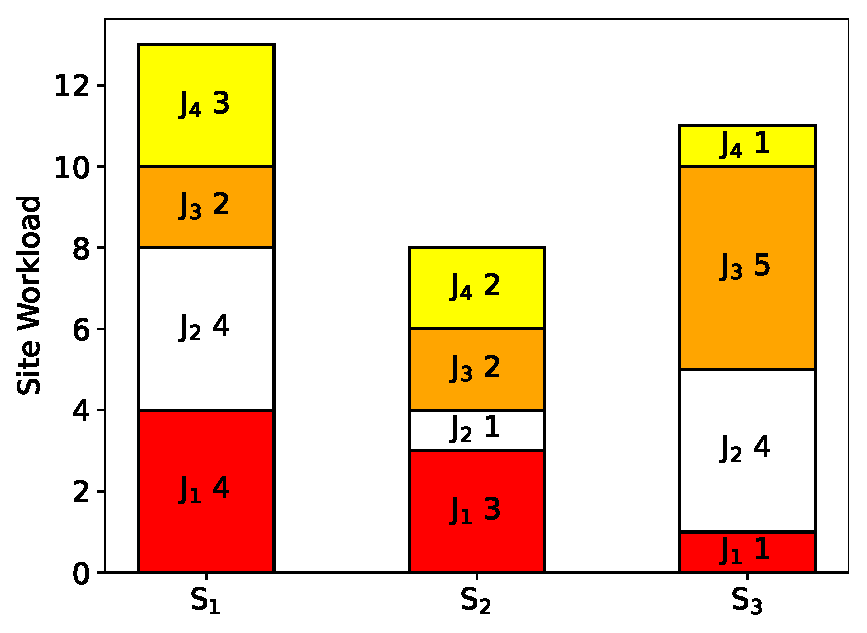
\includegraphics[width=\textwidth]{Image2/Example_1.eps}
        \caption{Indexed Scheduling}
        \label{fig_first_case}
    \end{subfigure}
    \hfill
    \begin{subfigure}[t]{0.48\textwidth}
        \centering
        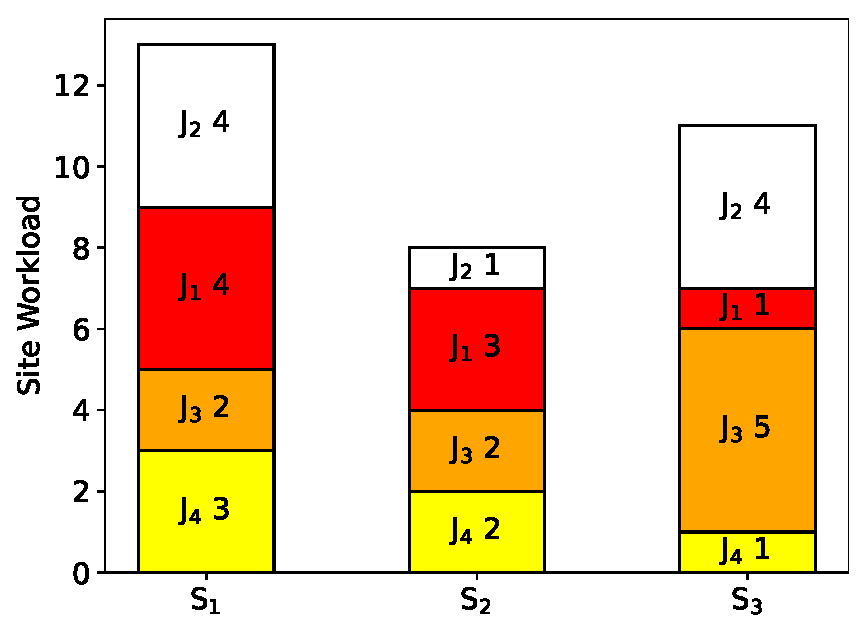
\includegraphics[width=\textwidth]{Image2/Example_2.eps}
        \caption{Optimal Scheduling without Task Transmission}
        \label{fig_second_case}
    \end{subfigure}
    
    \vspace{1.5em} % 👈 这里是关键：空行代表换行，\vspace 增加上下两行之间的间距
    
    % ========== 第二行 ==========
    \begin{subfigure}[t]{0.48\textwidth}
        \centering
        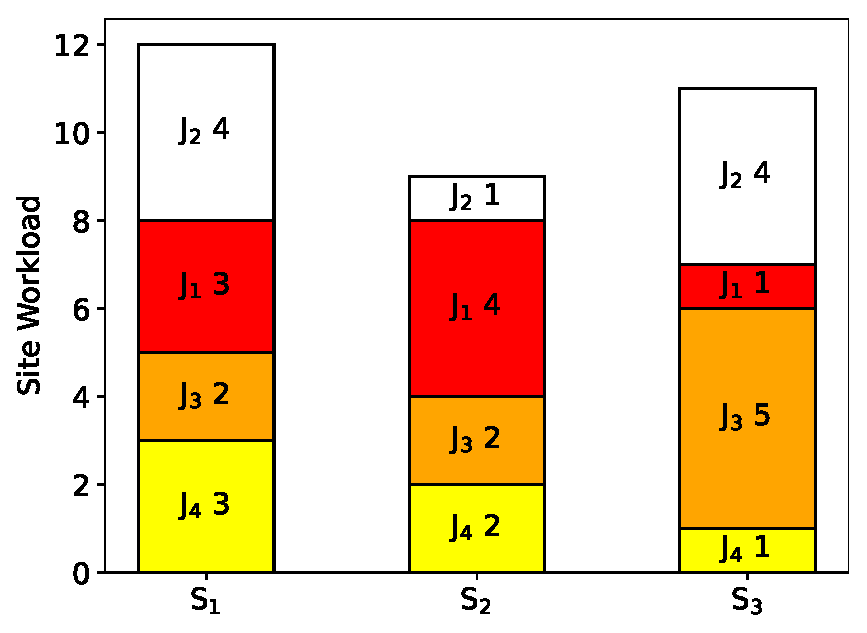
\includegraphics[width=\textwidth]{Image2/Example_3.eps}
        \caption{Optimal Transmission under Execution Order of Fig. \ref{fig_second_case}}
        \label{fig_third_case}
    \end{subfigure}
    \hfill
    \begin{subfigure}[t]{0.48\textwidth}
        \centering
        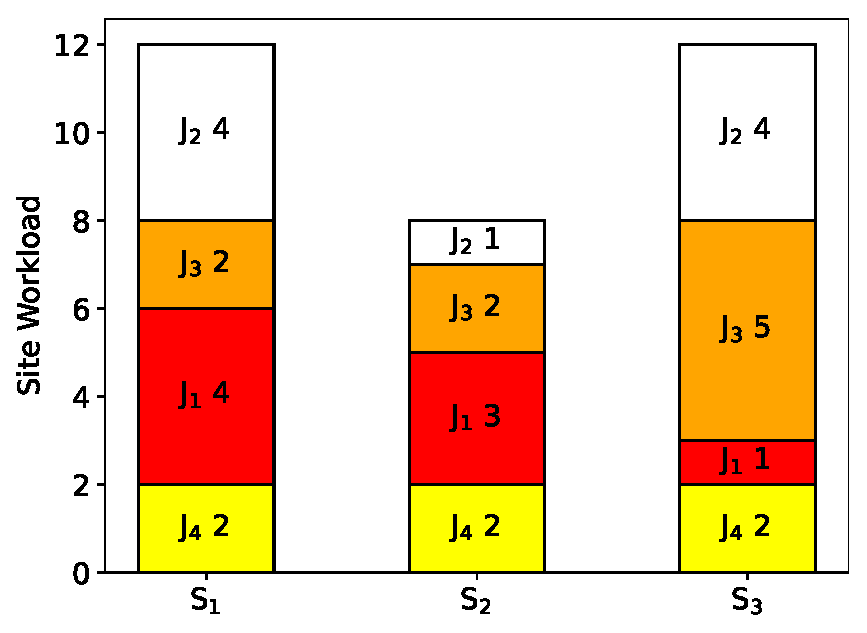
\includegraphics[width=\textwidth]{Image2/Example_4.eps}
        \caption{Optimal Scheduling with Task Transmission}
        \label{fig_fourth_case}
    \end{subfigure}
    
    \caption{Motivating Example} 
    \label{fig:Motivate_example}
\end{figure*}

Fig. \ref{fig:Motivate_example} provides a motivating example of the problem with four jobs $J_1$, $J_2$, $J_3$ and $J_4$ in three geo-distributed data centers (sites) $S_1$, $S_2$ and $S_3$. All jobs are submitted at time $0$. For simplicity, we assume that each task of any job requires one computing slot and takes one time unit to process, and each site has one computing slot only. Fig. \ref{fig_first_case} shows the initial task distribution of each job among the three sites. The response time of a job is decided by the completion time of its last task across all sites. Obviously, different execution orders of the jobs can change the completion times of their tasks and result in different job response times. If the jobs are simply scheduled in the order of their indices (which, for example, represents their submission order), jobs $J_1$, $J_2$, $J_3$ and $J_4$ will complete at time $4$, $8$, $10$ and $13$, respectively, so the total job response time is $4+8+10+13=35$ time units. The optimal job execution order without task transmission is $\langle J_4, J_3, J_1, J_2 \rangle$ as shown in Fig. \ref{fig_second_case}, and the resultant total job response time is $3+6+9+13=31$ time units, which is 4 time units better than the first schedule. 

Suppose that with utilization of network resources, the input data of one task is allowed to be transferred between sites and it takes one time unit to arrive at the destination. Under the job execution order of Fig. \ref{fig_second_case}, the optimal transmission can decrease the total job response time to 29 time units. For example, we can transfer one task of $J_1$ from site $S_1$ to $S_2$, as shown in Fig. \ref{fig_third_case}. This task will arrive at site $S_2$ at time $1$ when the slot of $S_2$ is processing a task of $J_4$ (and $J_4$ is scheduled earlier than $J_1$ in the execution order), so the task transferred can be treated as a local task of $J_1$ at site $S_2$ initially. Consequently, $J_4$, $J_3$, $J_1$ and $J_2$ will complete at time $3$, $6$, $8$ and $12$, respectively, and the total job response time is $3+6+8+12=29$ time units. In our example, the optimal solution is to transfer one task of $J_4$ from site $S_1$ to $S_3$ while modifying the job execution order to be $\langle J_4, J_1, J_3, J_2 \rangle$, as shown in Fig. \ref{fig_fourth_case}. This results in the total job response time of $2+6+8+12=28$ time units, which is even better than the schedule in Fig. \ref{fig_third_case}.

%The problem size (the transmission number limit in particular) of the motivating example is relatively small, and hence the performance disparity among different approaches is not substantial. Nevertheless, it reveals some interesting phenomena. %First, the optimal transmission of the task lies in $J_4$ which has the highest priority. This suggests that jobs with higher priorities in scheduling also tend to have high priorities on network resource usage: transferring out a task at the head of the scheduling queue has higher potential of bringing forward the procession start time of more tasks, which raises the probabilities that some jobs could finish earlier (if their completion times are dependent on their tasks at this site).
%impacting more jobs' completion time at the transmission source site and thereby their global completion time.  at the site where the transmission begins
The above example illustrates some interesting phenomena. First, job execution order and task transmission have mutual influence. The optimal execution order of jobs can change after task transmissions are performed: both execution orders in Figs. \ref{fig_second_case} and \ref{fig_fourth_case} achieve the optimal total job response times given the respective task transmissions, but $J_1$ and $J_3$ are swapped in the execution order after a task is transferred in Fig. \ref{fig_fourth_case}. Vice versa, different job execution orders have different optimal task transmissions: the optimal transmission changes after we modify the job execution order from $\langle J_4, J_3, J_1, J_2 \rangle$ (Fig. \ref{fig_third_case}) to $\langle J_4, J_1, J_3, J_2 \rangle$ (Fig. \ref{fig_fourth_case}). Second, the transmission in the optimal solution is from site $S_1$ to $S_3$, while the site with the lowest load is $S_2$. This indicates that the transmissions that minimize the total job response time can differ from the one that focuses on load balancing, so traditional load balancing techniques may not be preferable in this efficiency-targeted scenario.

\section{System Model}
\label{sec:model}
Consider a system consisting of $m$ separate geo-distributed sites: $\mathcal{S} = \{S_1, S_2, ..., S_m\}$. Each site $S_j$ has compute resources with capacity $u_j$, which can be interpreted as the volume of computing slots available. A set of $n$ jobs $J_1, J_2, ..., J_n$ are submitted to run in the system. Each job $J_i$ consists of tasks that require distinct data partitions and can run in parallel. For simplicity, we assume that each task takes one computing slot to process. In big data processing frameworks, tasks of the same job typically process data partitions of the same size \cite{shvachko2010hadoop, shanahan2015large_spark}, so they would take similar times to process. We denote the processing time of a task in each job $J_i$ as $l_i$, which can be estimated by the historical execution records of the job or sampling-based learning, which proactively samples a small fraction of the tasks in the job to make an estimate~\cite{jajoo2022slearn}.
A job is completed when all of its tasks are completed.

The data partitions required by the tasks of each job are originally distributed among the sites. Due to data locality consideration, each task is initially restricted to be executed at a certain site where its input data is available. Therefore, the computational demand of a job $J_i$ on site $S_j$ can be modeled as the number of its tasks that can run only on $S_j$ initially. We represent the computational demands of all jobs across all sites as a matrix $D_{n \times m}$, where each element $d_{ij}$ denotes job $J_i$'s computational demand on site $S_j$.%\footnote{Throughout this paper, we shall use capital letters to represent matrices as well as arrays, and use the corresponding small letters to stand for the elements therein.} 

Suppose the sites in the system are connected by networks, which can be used to transfer data and hence tasks from one site to another. The network resources in the system is denoted by a matrix $B_{m \times m}$, where each element $b_{ij}$ represents the bandwidth available on the link from site $S_i$ to site $S_j$. $b_{ij}$ is set to 0 if there is no direct link between $S_i$ and $S_j$. Let $r_k$ denote the size of a data partition of job $J_k$, then a task of $J_k$ takes $r_k/b_{ij}$ time to transfer from site $S_i$ to site $S_j$ (if $b_{ij}=0$, this time is defined to be infinite). For simplicity, we assume that the transmissions on each link are carried out sequentially. That is, if there is an ongoing transmission on the link, a new transmission has to wait and its arrival time at the destination site will be delayed.
% then transferring a single task of $J_k$ from site $S_i$ to $S_j$ takes $r_k/b_{ij}$ time
% it takes $r_k/b_{ij}$ time to transfer a single task (and its input data) of $J_k$ from site $S_i$ to $S_j$ (if $b_{ij}=0$, this time is defined to be infinite). 
%  job $J_k$ from site $S_i$ to $S_j$ is $r_k/b_{ij}$ (if $b_{ij}=0$, this time is defined to be infinite). Note that if there are ongoing transmission(s) on the link, a new transmission has to wait and its arrival time will be delayed.
\begin{table}[t]
  \caption{Summary of Notations}
  \label{tab:Notation}
  \centering
  \begin{tabularx}{\linewidth}{lX}
    \toprule
    \textbf{Notation} & \textbf{Definition} \\
    \midrule
    $\mathcal{S} = \{S_1, S_2, \dots, S_m\}$ & Set of sites \\
    $U=\{u_1, u_2, \dots, u_m\}$ & Compute resource capacities of individual sites \\
    $\{J_1, J_2, \dots, J_n\}$ & Set of jobs \\
    $D_{n \times m}$ & Compute resource demands \\
    $B_{m \times m}$ & Network resource availability \\
    $\{l_1, l_2, \dots, l_n\}$ & Task processing times of individual jobs \\
    $\{r_1, r_2, \dots, r_n\}$ & Data partition sizes of individual jobs \\
    \bottomrule
  \end{tabularx}
\end{table}

We study the problem of deriving an execution order of jobs and a set of task transmissions between sites, so that the total job response (completion) time of all jobs is minimized. %\textcolor{red}{Note that the response time of each job is the time span from its arrival (which is a constant) to its completion, so minimizing the total response time is equivalent to minimizing the total completion time.} 
The key notations used in this paper are summarized in Table \ref{tab:Notation}. For simplicity, we use $[x]$ to represent the set $\{1, 2, \dots, x\}$ for a positive integer $x$. Note that although the above model is formulated in a static setting, it can be easily extended to address online scenarios by dynamically capturing snapshots of job demand distributions and system resources. %Here $\langle J_{1}', J_{2}',...,J_{n}'\rangle$ is a sequence where each element $J_{i}'$ denotes the $i$-th job to be processed. $T$ is a three-dimensional matrix and $t_{ijk}$ refers to the number of tasks of $J_i$ to be transferred from $S_j$ to $S_k$. 

\section{Workload-Aware Selection with Transmission}
\label{sec:WAST}

\subsection{Optimizing the Completion Time of a Single Job}
\label{sec:single1}
We start by considering the subproblem of how to utilize network resources in the system to minimize the completion time of a single job. This subproblem can be formulated as follows: Given some workloads and task transmissions already scheduled in the system, and a job $J_k$ with task processing time $l_k$, data partition size $r_k$ and initial demand distribution $d_{k1}, d_{k2}, \dots, d_{km}$ across the $m$ sites, % associated with scheduled jobs from the previous iteration(s)
we would like to determine a set of task transmissions for $J_k$ so that its job completion time can be minimized.
%To describe the state of the system load prior to scheduling $J_k$, we

We use a sequence of arrays $W_1, W_2, \dots, W_m$ to represent the workload already scheduled for each computing slot at each site, where the workload of a slot refers to the total processing time of all tasks assigned to it (i.e., the time when this slot will become available). Each $W_i$ is an array whose length is the number of computing slots at site $S_i$, and each element $w_{ij}$ in $W_i$ represents the scheduled workload of the $j$-th slot at $S_i$. In addition, we use a matrix $T_{m \times m}$ to represent the usage of network resources by the task transmissions already scheduled, where $t_{ij}$ records the time when the link from site $S_i$ to site $S_j$ will complete the scheduled transmissions and become available.% Initially, all $b_{ij}'$s are set to 0. Once a transmission is scheduled, its transmission time will be added to the corresponding entry in $T$.

To avoid the complex interaction between task transmissions and executions and simplify the problem model, we assume that every transferred task will arrive at its destination site before any computing slot at that site becomes available. % \sout{at that site starts to process tasks of subsequent jobs in the execution order}. \sout{This ensures that the tasks of the job (including transferred ones) are processed continuously at each site} 
This ensures that the transferred tasks can be processed continuously at their destination sites together with the tasks originally available there, which simplifies the modeling of job completion time. Based on this, we model the completion time of job $J_k$ as follows. Suppose a matrix $X_{m \times m}$ represents the task transmissions of job $J_k$, where each element $x_{ij}$ refers to how many tasks of $J_k$ are to be transferred from site $S_i$ to site $S_j$. Naturally, each $x_{ij}$ is greater than or equal to $0$. In particular, for each site $S_i$, we define $x_{ii}=0$. We use an array $Y$ of length $m$ to represent the computational demands at the $m$ sites after all the transmissions in $X$ are performed. Each element $y_i$ refers to the number of tasks to be executed at site $S_i$ after the transmissions, and is given by:%. Obviously, the variables in $X$ and $Y$ are integers and for them we have:
\begin{equation}
    \forall i \in [m],\quad y_i = d_{ki} + \sum_{j=1}^m x_{ji} - \sum_{j=1}^m x_{ij}.
\label{eq:constraint1}
\end{equation}

Recall that we assume each task transmission to arrive at its destination site before any computing slot at that site becomes available. Thus, all the $y_i$ tasks of job $J_k$ to be executed at site $S_i$ can be scheduled by iteratively assigning each task to the slot of the lowest workload in $S_i$. Let $w_{ij}^{(t)}$ denote the workload of the $j$-th slot in site $S_i$ after $t$ tasks of $J_k$ are assigned to the slots at $S_i$. $w_{ij}^{(t)}$ can be computed iteratively as follows:% \[
% \begin{aligned}
% \text{Initialization: }&\forall j \in [u_i], \text{ } w_{ij}^{(0)} = w_{ij},\\
% \text{for each } & t = 1, \;2, \;\dots, \;y_i:\\
% %\text{find the slot $p$ with the lowest workload: }\\
% %p = \text{any } &\text{element of }\argmin_{1 \le j \le u_i} w_{ij}^{(t-1)}, \\
% \forall j \in [u_i],& w_{ij}^{(t)} =
% \begin{cases}
% w_{ij}^{(t-1)} + l_k, & j = \argmin_{1 \le p \le u_i} w_{ip}^{(t-1)}, \\
% w_{ij}^{(t-1)}, & else.
% \end{cases} \\
% \end{aligned}
% \]
%\begin{equation*}
%\forall j \in [u_i], \text{ } w_{ij}^{(0)} = w_{ij},
%\end{equation*}
\begin{multline}
\!\!\!\!\!\!\forall j \in [u_i], \;\;\; 
w^{(t)}_{ij} =
\begin{cases}
w_{ij}, \qquad \qquad \, t=0 \\
w^{(t-1)}_{ij} + l_k, 
\;\;\; j = \argmin_{p \in [u_i]} w^{(t-1)}_{ip}, \\
w^{(t-1)}_{ij}, 
\qquad \;\;\; j \neq \argmin_{p \in [u_i]} w^{(t-1)}_{ip}, 
\end{cases}
\nonumber
\end{multline}
where in each iteration, a task is assigned to the slot of the lowest workload ($\argmin_{p \in [u_i]} w_{ip}^{(t-1)}$) and its workload then increases by $l_k$, while other slots are kept unchanged. Ties are broken arbitrarily if multiple slots have the same lowest workload.
Based on this, the time when all $y_i$ tasks complete execution at site $S_i$ can be estimated as a function $f(W_i, y_i)$:
\[
f(W_i, y_i) =
\begin{cases}
0, & y_i = 0, \\
\min_{j \in [u_i]}(w_{ij}^{(y_i-1)})+l_k,  & y_i > 0,
\end{cases}
\]
which gives the completion time of the last task at $S_i$.
Note that function $f$'s inputs and outputs cannot be captured by any closed-form expression. %Therefore, given any $y_i$, the completion time of all $y_i$ tasks at site $S_i$ can be derived based on the computation above. 
The objective of optimizing the job completion time of $J_k$ (i.e., $\max_{i \in [m]} f(W_i,y_i)$ --- the completion time of its last task across all sites) can be achieved by searching for the best task transmissions $X$ between sites, which decide the computational demands $Y$ at different sites and hence job $J_k$'s completion time. 
%Not working: Here we suppose tasks are added one slot by one slot.
%If there is a deep low workload at some slot, it may need multiple tasks to be added to it consecutively.
%In this circumstance, given how many tasks are present at a site $S_i$ (tasks transferred from other sites will arrive at the time when all local slots are still busy processing tasks of jobs with prior execution order or tasks of the same job, thus they could be treated in a similar way as local demand), we could add tasks  using a step-by-step manner, and the estimated job response time on a site $S_i$ can be expressed as follows:
%derive the resultant job response time on $S_i$ given any $Y_i$: %WLOG, suppose the computing slots in $S_i$ has a non-decreasing workload $W_{i0} \leq W_{i1} \leq ...... \leq W_{iU_i}$, then the estimated job response time on site $S_i$ is a integer function of $Y_i$:


%It is important to determine the bound of $X$ and $Y$ before searching starts, and there are multiple factors restricting the bounds. Suppose that the current job is $J_k$: first, a transmission could start only if there is existing demand on the site, so each $x_{ij}$ and $y_i$ has a lower bound $-d_{ki}$; second, transmission could only happen when the starting site's estimated local JRT is larger than that of the destination site, because a valid transmission will narrow instead of deteriorate the gap of local JRT between any two sites. This restricts the upper limit on half of the elements in $X$ to be zero and lower limit to be zero on the other half. Third, to ensure that a transmission will arrive in time, the existing transmission delay of the link plus the unit transmission time cost should be less than or equal to the minimum workload of the slot in the destination site. This further controls the upper limit of the elements in $X$. Finally, each site could receive tasks as long as its local JRT is still smaller than the global JRT without transmission, which gives upper bounds on each element in $Y$. Together, these constraints derive the upper and lower bounds of $X$ and $Y$; To facilitate the representation, we use $A$ and $C$ to record the upper bound in $X$ and $Y$, respectively. The algorithm \ref{alg:Single1} describes the basic approach to find the minimum JRT that current job $J_k$ is possible to reach. The algorithm first computes the lower and upper bounds for variables in $X$ and $Y$ as well as the estimated local JRT given how many tasks are added to or removed from each site, then start a program to minimize the maximum local JRT, a.k.a., global JRT.

It is essential to determine the bounds of $X$ before starting the search. 
%as they are restricted by multiple factors. 
An excessively tight bound can limit the potential benefit of task transmissions in reducing the job completion time, whereas an excessively loose bound may give rise to task transmissions that fail to reach the destination sites in time, thereby introducing additional delays in the job completion time. %As discussed, we \textcolor{red}{hope} each task to arrive at its destination site when no computing slot of that site has started processing the subsequent jobs. \sout{, and we require it to be no later than the lowest workload among all slots after $d_{kj}+x_{ij}-1$ tasks are assigned to $S_j$. Such modeling of the task transmission requirement assumes that at least $d_{kj}$ tasks are present at the destination site $S_j$ when the first transmission from site $S_i$ arrives, and does not account for potential task transmissions out of site $S_j$ as well as transmissions to site $S_j$ from sites other than $S_i$}
%the arrival time of the last transmission is $t_{ij} + x_{ij}\cdot r_k/b_{ij}$, and 
Suppose $x_{ij}$ tasks are to be transferred from site $S_i$ to site $S_j$. Then, the completion time of the last task will be at least $t_{ij} + x_{ij}\cdot r_k/b_{ij} + l_k$ (when it is processed immediately after arrival), and we require this last task to finish before the job completion time:
\begin{multline}
\forall i \in [m], \; j \in [m], \;
t_{ij} + \frac{x_{ij} \cdot r_k}{b_{ij}} + l_k \le \max_{i \in [m]} f(W_i,y_i).
\label{eq:constraint_t}
\end{multline}

In addition, the number of tasks transferred out of a site cannot exceed the number of tasks it holds initially, which imposes another upper bound on $\sum_{j=1}^m x_{ij}$ at each site $S_i$:
\begin{equation}
    \forall i \in [m], \quad 0 \leq \sum_{j=1}^m x_{ij} \leq d_{ki}.
\label{eq:constraint_sum}
\end{equation}
%Constraint (\ref{eq:constraint_sum}) ensures that the sum of the first and third terms ($d_{ki} -\sum_{j=1}^m x_{ij}$) in equation (\ref{eq:constraint1}) is nonnegative, which provides implicit guarantees that the elements in $Y$ are nonnegative. 

Constraints (\ref{eq:constraint_t}) and (\ref{eq:constraint_sum}) collectively define the upper bounds of the elements in $X$. Therefore, we can define a program to search for task transmissions $X$ under constraints (\ref{eq:constraint1}), (\ref{eq:constraint_t}) and (\ref{eq:constraint_sum}) to optimize the job completion time $\max_{i \in [m]} f(W_i,y_i)$. %which decides the number of tasks after transmissions on each site $Y$, and hence job $J_k$'s response time (using function $f$). }% Since each element in $Y$ is a linear combination of some elements in $X$, its upper bounds are implicitly determined by $X$.
%Second, a valid transmission should only reduce the disparities between the task completion times at different sites. Hence, transmissions should not be performed from site $S_i$ to site $S_j$ if the estimated task completion time at the source site $f(S_i, d_{ki})$ is no later than that at the destination $f(S_j, d_{kj})$ when all tasks are processed without transmissions. This imposes an upper bound of zero on half of the elements in $X$:
%The constraints (\ref{eq:constraint_Xbound}), (\ref{eq:constraint3}) and (\ref{eq:constraint4}) above collectively define the feasible upper bounds of elements in $X$. Since each element in $Y$ is a linear combination of some elements in $X$, its upper bound are implicitly determined by $X$. %For notational convenience, we denote the upper bounds of $X$ derived by the constraints above as a matrix $A$, where each element $a_{ij}$ represents the upper bound of $x_{ij}$ in $X$:
If multiple transmission matrices $X$'s produce the same minimum job completion time, we choose the $X$ with the least total number of task transmissions. The rationale is to minimize the network resource usage and make more network resources available to other jobs.
% with minimized $\sum_{i=1}^m \sum_{j=1}^m x_{ij}$ are returned.

%If any $Y_i=0$, the resultant JRT of $S_i$ is its initial local JRT. Similarly, initially, the local demand of current job across all sites could be simply placed one by one(note that with the principle mentioned above, there is no need to consider transmissions of jobs with higher priority, because they must have arrived and been in process before tasks of the current job start to proceed), each time selecting the slot with the lowest workload. After this, we could obtain the estimated local JRT of the current job across each site. We define a transmission using a tuple $E(J_i, S_j, S_k)$, representing a transmission's belonging job, start site and destination site, respectively. A valid transmission should satisfy some basic conditions: 

\subsection{Transformation into ILP}
\label{sec:transformation}
The program in Section \ref{sec:single1} cannot be solved directly by popular optimization solvers owing to the discrete function $f$, which 
%As mentioned previously, due to various workload conditions at different sites, the relationship between $f$'s inputs and outputs 
cannot be captured by any closed-form expression. % For example, after a task is assigned to some site $S_j$, it is possible that the task completion time of $S_j$ increases or remains unchanged. 
%seems to provide a complete solution for the single-job case. However, it
In order to make the program solvable, we transform it into solving multiple Integer Linear Programs (ILP) that are supported by popular solvers. To facilitate presentation, we refer to the completion time of the last task at a site $S_i$ as "the completion time at site $S_i$". We compute and record the completion times $f(W_i, y_i)$ at each site $S_i$ using the method introduced in Section \ref{sec:single1}, for increasing number of tasks $y_i$ scheduled at site $S_i$ starting from $y_i=0$. %\sout{In particular, $f(W_i, 0)$ is set to 0 for each site $S_i$.} 
The calculation ends at the lowest $y_i$ value where the resulting $f(W_i, y_i)$ at site $S_i$ exceeds the job completion time when all tasks are executed locally without transmission, i.e., $\max_{i\in[m]}f(W_i, d_{ki})$. 

Note that these $f(W_i, y_i)$ values include all possible completion times at each site that $J_k$ can produce, and they are non-decreasing with respect to $y_i$ since adding a new task can never reduce the completion time at a site. With these $f(W_i, y_i)$ values, given any target job completion time $z$, the maximum number of tasks $c_i$ that each site $S_i$ can process (to keep its completion time within this target) can be derived as $c_i = \max\{p \mid f(W_i, p)\leq z\}$. Thus, the target $z$ can be converted to an array of upper bounds $c_1, c_2, \dots, c_m$ for the elements $y_1, y_2, \dots, y_m$ in $Y$. Hence, the problem of determining ``whether the job $J_k$ can achieve a target job completion time $z$ using task transmissions'' can be transformed to determining whether task transmissions can be performed to bound the elements in $y_1, y_2, \dots, y_m$ by $c_1, c_2, \dots, c_m$. The latter can be formulated as an ILP, because its constraints are linear and the elements in $X$ and $Y$ are integers. Furthermore, the minimum job completion time that $J_k$ can achieve must be among all the $f(W_i, y_i)$ values. Therefore, we can sort all values $f(W_1, 0)$, $f(W_1, 1), \dots, f(W_1, c_1), f(W_2, 0), f(W_2, 1), \dots, f(W_2, c_2)$, $\dots, f(W_m, 0), f(W_m, 1), \dots, f(W_m, c_m)$ to form an array $\psi$. Then, the minimum job completion time of $J_k$ can be found by a binary search in $\psi$ and solving multiple ILPs.
%In this circumstance, the result $P_{it}$ is discarded, and the computation for the site ends.% Once after a new task is added to a site and the corresponding job response time exceeds the threshold,
%We compute the completion times at each site given different numbers of tasks and record them in $m$ arrays, namely $P_1, P_2, \dots, P_m$. More specifically, each element $p_{ij}$ records the completion time at site $S_i$ if $j$ tasks of $J_k$ are processed at $S_i$. \textcolor{red}{The first element $p_{i0}$ of each array $P_i$ is set to 0.} The method of computing the array $P_i$ is based on the approach used for calculating $w_{ij}^{(t)}$s in Section \ref{sec:single1}. We record $\min_{1\leq j \leq u_i}w_{ij}^{(t-1)} + l_k$ for each $t=1, 2,\dots$ as $p_{it}$. The computation ends at the lowest $t$ value where the resulting completion time $\min_{1\leq j \leq u_i}w_{ij}^{(t-1)} + l_k$ at site $S_i$ exceeds the original job response time (i.e., the job response time when all tasks are executed locally without transmission). %In this circumstance, the result $P_{it}$ is discarded, and the computation for the site ends.% Once after a new task is added to a site and the corresponding job response time exceeds the threshold,

%Note that the array set $P_1, P_2, \dots, P_m$ stores all possible completion times at each site that $J_k$ can produce, and each array is guaranteed to be non-decreasing with respect to their indices since adding a new task can never reduce the completion time at a site. With this array set, given any target job response time $z$, the maximum number of tasks that a site $S_i$ can process (to keep its corresponding completion time within this target) can be derived by checking array $P_i$. \textcolor{red}{More specifically, suppose that the number of elements of array $P_i$ is $P_i.size$, this maximum number is $\argmax_{0\leq j < P_i.size}p_{ij}\leq z$.} Thus, the target can be converted to an array of upper bounds $c_1, c_2,\dots,c_m$ for the elements $y_1, y_2, \dots, y_m$ in $Y$. Hence, the problem "whether the job $J_k$ could achieve this target job response time using task transmissions" is equivalent to determining whether task transmissions can be performed to bound the elements in $Y$ by $C$. The latter can be formulated as an ILP, because its constraints are linear and the elements in $X$ and $Y$ are integers. Furthermore, the minimum job response time that $J_k$ can achieve must be in the array set $P_1, P_2, \dots, P_m$. Therefore, we can consolidate all elements in $P_1, P_2, \dots, P_m$, eliminate duplicates if any, and sort them to derive an array $\psi$, and the minimum job response time of $J_k$ can be found by a binary search in $\psi$ and solving multiple ILPs.%(note that by the transformation above we eliminated constraints using function $f$)


%is the optimal solution $J_k$ could possibly achieve. Every entry in $Y$ should at

%that fall below the minimum local JRT are discarded, as they are irrelevant or infeasible. We then utilize binary search to obtain the minimum JRT bound from $JRT_p$ and return the transmission $X$ under this JRT bound. By such modification, we replace Algorithm \ref{alg:Single1} with a series of ILP instances to efficiently identify the minimum achievable JRT for $J_k$. The procedure is elaborated in Algorithm \ref{alg:Single2}. 
% 请确保在 LaTeX 文件的导言区（Preamble）引入了该宏包：
% \usepackage[linesnumbered,ruled,vlined]{algorithm2e}

\begin{algorithm}[t]
\caption{Optimizing the Completion Time of a Single Job}\label{alg:Single2}

    \KwIn{A set of sites $\mathcal{S}$ with compute capacities $U$ and network resources $B$; a job $J_k$ to be scheduled with task processing time $l_k$, data partition size $r_k$ and computational demand distribution $d_{k1}, d_{k2}, \dots, d_{km}$; current workload $W_1, W_2, \dots, W_m$ and network usage $T$;}
    \KwOut{$J_k$'s optimal job completion time and task transmissions;}
    \BlankLine

    Compute and record $f(W_i, y_i)$'s for each site $S_i$ with increasing $y_i$ until $f(W_i, y_i) \geq \max_{i\in[m]}f(W_i, d_{ki})$, using the method in Section \ref{sec:single1}\;
    Merge and sort all $f(W_i, y_i)$ values to form an array $\psi$\;
    % Collect all possible task completion times that each site can reach, record them in arrays $P_1, P_2, \dots, P_m$; merge and sort them into an array $\psi$; remove duplicate elements from $\psi$;
    $low=1$; $high=\psi.size$; $opt = 0$\;
    \BlankLine

    \While{$low < high$}{
        $middle = \lfloor (low + high)/2\rfloor$\;
        $c_i = \max\{p \mid f(W_i, p)\leq \psi[middle]\}$, for each $i \in [m]$\;
        \BlankLine
        
        Minimize $\sum_{i=1}^m\sum_{j=1}^m x_{ij}$, subject to:\;
        \quad $\forall i \in [m], j \in [m],\; t_{ij} + \frac{x_{ij}*r_k}{b_{ij}} + l_k \leq \psi[middle]$;\;
        \quad $ \forall i \in [m],\; 0 \leq \sum^m_{j=1}x_{ij} \leq d_{ki}$;\;
        \quad $ \forall i \in [m],\; y_i = d_{ki} + \sum_{j=1}^m x_{ji} - \sum_{j=1}^m x_{ij}$;\;
        \quad $\forall i \in [m],\; y_i \leq c_i$;\;
        \quad all $x_{ij}$'s and $y_i$'s are non-negative integers;\;
        \BlankLine
        
        \eIf{the above ILP is feasible and admits a solution}{
            $opt = \psi[middle]$\;
            $X \leftarrow x_{ij}$'s in the solution of the above ILP\;
            $high = middle - 1$\;
        }{
            $low = middle + 1$\;
        }
    }
    \BlankLine
    \Return $opt$, $X$\;
\end{algorithm}

% \begin{algorithm}[t]
% \caption{Optimizing the Completion Time of a Single Job}
% \label{alg:Single2}
% \begin{algorithmic}[1]
% \STATE \textbf{Input}: A set of sites $\mathcal{S}$ with compute capacities $U$ and network resources $B$; a job $J_k$ to be scheduled with task processing time $l_k$, data partition size $r_k$ and computational demand distribution $d_{k1}$, $d_{k2}, \dots, d_{km}$; current workload $W_1, W_2, \dots, W_m$ and network usage $T$;
% \STATE \textbf{Output}: $J_k$'s optimal job completion time and task transmissions;
% \STATE \textbf{Initialization}: Compute and record $f(W_i, y_i)$'s for each site $S_i$ with increasing $y_i$ until $f(W_i, y_i) \geq \max_{i\in[m]}f(W_i, d_{ki})$, using the method in Section \ref{sec:single1}; merge and sort all $f(W_i, y_i)$ values to form an array $\psi$;%Collect all possible task completion times that each site can reach, record them in arrays $P_1, P_2, \dots, P_m$; merge and sort them into an array $\psi$; remove duplicate elements from $\psi$; %remove elements below the ideal bound derived under the infinite bandwidth assumption from $\psi$. 
% % \STATE Compute $X$'s upper bound $A$ based on the following constraints:
% % \STATE$\forall i \in [m], j \in [m]: 0 \leq x_{ij} \leq d_{ki}$;
% % \STATE$\forall i \in [m], j \in [m]: f(S_i,d_{ki}) \leq f(S_j, d_{kj}) \xrightarrow{} x_{ji} \leq 0$;
% % \STATE$\forall i \in [m], j \in [m]: T_{ij} + \frac{x_{ij}*r_k}{b_{ij}} \leq \min(w^{\max(0, (x_{ij}-1))}_j)$;
% \STATE $low=1$; $high=\psi.size$; $opt = 0$;
% \WHILE {$low < high$}
% \STATE $middle = \lfloor (low + high)/2\rfloor$;
% \STATE $c_i = \max\{p \mid f(W_i, p)\leq \psi[middle]\}$, for each $i \in [m]$;%Update $Y$'s upper bound $C$ based on $\psi_{middle}$ and $P_1, P_2, \dots, P_m$;
% \STATE Minimize $\sum_{i=1}^m\sum_{j=1}^m x_{ij}$, subject to:
% %\STATE \quad Minimize $max\_JRT$, subject to:
% %\STATE $\quad \forall i \in [m]: max\_JRT \geq JRT(y_i)$;

% %\STATE \quad$ \forall i \in [m], j\in [m]: 0 \leq x_{ij} \leq a_{ij}$;
% \STATE \quad $\forall i \in [m], j \in [m],\; t_{ij} + \frac{x_{ij}*r_k}{b_{ij}} + l_k \leq \psi[middle]$;
% \STATE \quad$ \forall i \in [m],\; 0 \leq \sum^m_{j=1}x_{ij} \leq d_{ki}$;
% \STATE \quad$ \forall i \in [m],\; y_i = d_{ki} + \sum_{j=1}^m x_{ji} - \sum_{j=1}^m x_{ij}$;
% \STATE \quad $\forall i \in [m],\; y_i \leq c_i$;
% \STATE \quad all $x_{ij}$'s and $y_i$'s are non-negative integers; 
% % \STATE \quad $\forall i \in [m], j \in [m], x_{ij} \in N^+$
% \IF{the above ILP is feasible and admits a solution}
% \STATE $opt = \psi[middle]$;
% \STATE $X \leftarrow x_{ij}$'s in the solution of the above ILP;
% \STATE$high = middle - 1$;
% \ELSE
% \STATE$low = middle + 1$;
% \ENDIF
% \ENDWHILE
% \STATE \textbf{return} $opt$, $X$;
% \end{algorithmic}
% \end{algorithm}

\begin{figure}[htbp]
  \centering
  %\resizebox{\linewidth}{!}{
\begin{tikzpicture}
[
    scale=0.65, 
    transform shape,
    %transform shape=false,
    % node distance=10mm and 22mm,
    % rect/.style={draw, rounded corners, minimum width=14mm, minimum height=9mm, align=center},
    % s/.style={circle, draw, thick, minimum size=9mm, align=center},
    % edge/.style={-Stealth, thick},
    % labsmall/.style={font=\small}
    node distance=1.5em and 3em,
    rect/.style={draw, rounded corners, minimum width=4em, minimum height=2.5em, align=center, font=\normalsize},
    s/.style={circle, draw, thick, minimum size=2.5em, align=center,, font=\normalsize},
    edge/.style={-Stealth, thick},
    labsmall/.style={font=\small}
]

% --- nodes: source, tasks (with vdots), sites (with vdots), sink

\node[rect] (SS1) {$S_1^{out}$};
\node[rect, below=of SS1] (SS2) {$S_2^{out}$};
\node[rect, below=of SS2] (SS3) {$S_3^{out}$};
\node[s, left=28mm of SS3] (s) {$s$};
\node[font=\Large, below=of SS3] (Tdots) {$\vdots$};
\node[rect, below=of Tdots] (SSm) {$S_m^{out}$};

\node[rect, right=35mm of SS1] (S1) {$S_1^{in}$};
\node[rect, below=of S1] (S2) {$S_2^{in}$};
\node[rect, below=of S2] (S3) {$S_3^{in}$};
\node[font=\Large, below=of S3] (Sdots) {$\vdots$}; 
\node[rect, below=of Sdots] (Sm) {$S_m^{in}$};
\node[s, right=28mm of S3] (t) {$t$};

% --- dashed vertical separators (optional, 改坐标可调整高度)
% \draw[dashed] ($(s)+(16mm,28mm)$) -- ($(s)+(16mm,-44mm)$);   % between source and T
% \draw[dashed] ($(S1)+(16mm,28mm)$) -- ($(S1)+(16mm,-44mm)$); % between S and sink

% --- edges: source -> tasks
\draw[edge] (s) -- (SS1) node [midway, above, sloped] {$d_{k1}$};
\draw[edge] (s) -- (SS2) node [midway, above, sloped] {$d_{k2}$};
\draw[edge] (s) -- (SS3) node [midway, above, sloped] {$d_{k3}$};
\draw[edge] (s) -- (SSm) node [midway, above, sloped] {$d_{km}$};

% --- edges: tasks -> sites (示例连接，按需改/增)
\draw[edge] (SS1) -- (S1);
\draw[edge] (SS1) -- (S2);
\draw[edge] (SS1) -- (S3);
\draw[edge] (SS2) -- (S1);
\draw[edge] (SS2) -- (S2);
\draw[edge] (SS2) -- (S3);
\draw[edge] (SS3) -- (S1);
\draw[edge] (SS3) -- (S2);
\draw[edge] (SS3) -- (S3);
\draw[edge] (SSm) -- (Sm);

% --- edges: sites -> sink
\draw[edge] (S1) -- (t)node [midway, above, sloped] {$c_{1}$};
\draw[edge] (S2) -- (t)node [midway, above, sloped] {$c_{2}$};
\draw[edge] (S3) -- (t)node [midway, above, sloped] {$c_{3}$};
\draw[edge] (Sm) -- (t)node [midway, above, sloped] {$c_{m}$};

\end{tikzpicture}
%}
\caption{The flow network}
\label{fig:flow_network}
\end{figure}

Algorithm \ref{alg:Single2} presents the details of optimizing the job completion time of job $J_k$. $\psi.size$ represents the number of elements in the array $\psi$. The algorithm first computes and records the possible completion times $f(W_i, y_i)$ at each site $S_i$ using the method introduced in Section \ref{sec:single1}. These values are then merged and sorted to form a new array $\psi$ which records the job completion times that $J_k$ can possibly achieve. Next, a binary search is applied to the array $\psi$ to find the optimal job completion time in $\psi$ as well as the transmissions required. The parameters $low$ and $high$ in the algorithm refer to the boundary indices of the binary search. In each iteration, the $middle$ index and bounds $c_1, c_2, \dots, c_m$ are updated, and the feasibility of an ILP is checked to decide whether the job completion time $\psi[middle]$ is achievable.
%, and elements that are either duplicated or below a certain threshold are removed from $JRT\_p$ to reduce computation overhead. Next, a binary search method is applied to $JRT\_p$ so that each time a time threshold in $JRT\_p$ is located. The upper bound $C$ of entries in $Y$ are updated using the threshold, and a new ILP is constructed to decide whether this threshold is achievable. After the binary search, the optimal job response time as well as the required transmission(s) can be found. Details of the algorithm are elaborated in Algorithm \ref{alg:Single2}. The parameters $low$ and $high$ in the algorithm refer to the left and right boundary indices of the binary search. $JRT\_p.size$ returns the number of elements in $JRT\_p$., during which elements duplicated and elements that fall below the ideal lower bound are removed

\subsection{Transformation into Minimum-cost Flow Problem}
\label{sec:flow}


% \begin{figure}[htbp]
%     \centering
% \includegraphics[width=\linewidth]{flow_network.tikz}
%     \caption{The flow network}
%     \label{fig:flow_network}
% \end{figure}
\begin{comment}
\begin{algorithm}[htbp]
\caption{Optimizing the Completion Time of a Single Job}
\label{alg:Single3}
\begin{algorithmic}[1]
\STATE \textbf{Input}: A set of sites $\mathcal{S}$ with compute capacities $U$ and network resources $B$; a job $J_k$ to be scheduled with task processing time $l_k$, data partition size $r_k$ and computational demand distribution $d_{k1}$, $d_{k2}, \dots, d_{km}$; current workload $W$ and network usage $T$;
\STATE \textbf{Output}: $J_k$'s optimal job response time and transmissions;
\STATE \textbf{Initialization}: Compute and record $f(W_i, y_i)$'s for each site $S_i$ with increasing $y_i$ until $f(W_i, y_i) \geq \max_{i\in[m]}f(W_i, d_{ki})$, using the method in Section \ref{sec:single1}; merge and sort all $f(W_i, y_i)$ values to form an array $\psi$; %remove elements below the ideal bound derived under the infinite bandwidth assumption from $\psi$. 

\STATE $low=1$; $high=\psi.size$; $opt = 0$;
\While {$low < high$}
\STATE $middle = \lfloor (low + high)/2\rfloor$;
\STATE $c_i = \max\{p \mid f(W_i, p)\leq \psi[middle]\}$, for each $i \in [m]$;
%\STATE Update the capacity of edge $(S^{in}_i, t)$ to be the new $c_i, i=1,2,\dots, m$;
\STATE Construct the flow network for $J_k$;
\STATE Solve the flow network while minimize the flow cost;
\If{the above flow network admits a total flow of $\sum_{i=1}^m d_{ki}$ units}
\STATE $opt = \psi[middle]$;
% \For {$i \in [m], j \in[m], j \neq i$}
% \STATE $x_{ij}=$ flow of edge $(S_i^{out}, S_j^{in})$;
% \EndFor
\STATE $x_{ij}=$ the flow amount on edge $(S_i^{out}, S_j^{in})$, for each $i,j \in [m]$ and $i \neq j$;
\STATE $x_{ii}=0$, for each $i \in [m]$;
\STATE$high = middle - 1$;
\Else
\STATE$low = middle + 1$;
\EndIf
\EndWhile
\STATE \textbf{return} $opt$, $X$;
\end{algorithmic}
\end{algorithm}
\end{comment}
%can be examined from a slightly different perspective: Each site $S_i$ has an initial number of tasks $d_{ki}$, and the number of tasks that each site could transfer to another site $S_j$ has an upper limit denoted by $t_{ij} + \frac{x_{ij}*r_k}{b_{ij}} \leq \min(w^{(d_{kj}+x_{ij}-1)}_j)$. The question is to find a set of transmissions so that site $S_i$'s final number of task $y_i$ falls below $c_i$. the objective becomes to find a set of flows that fall below their corresponding flow capacities (including the capacities for each link in the network and capacities for each site $c_i$). 

Algorithm \ref{alg:Single2} solves the problem, but its computational complexity could raise concerns. 
%Under the transformation in the last section, the problem of searching for the minimum job response time of a single job is decomposed into multiple ILP feasibility problems, which 
ILP is NP-hard in general. If the solution space becomes huge (e.g., the job has thousands of tasks unevenly spread across tens of geo-distributed sites), solving the ILP can incur intolerable computational overhead. To improve the algorithm's efficiency, we further transform the ILP problem in lines 8-13 of Algorithm \ref{alg:Single2} to a minimum-cost flow problem in a bipartite flow network shown in Fig.~\ref{fig:flow_network}. The flow network has a source node $s$, a sink node $t$, a set of $m$ nodes on the left side and a set of $m$ nodes on the right side. To facilitate exposition, we use $S^{out}_i$ and $S^{in}_i$ to represent the $i$-th node on the left and right sides, respectively. A set of $m$ edges with cost 0 connects the source node $s$ to the $m$ nodes on the left, and the capacity of each edge $(s, S_i^{out})$ is set to $d_{ki}$. In addition, a set of $m\times m$ edges connects the $m$ nodes on the left to the $m$ nodes on the right. The capacity of each edge $(S_i^{out},S_j^{in})$ where $i\neq j$ is set to the upper bound of $x_{ij}$ given in line 9 of Algorithm \ref{alg:Single2} (where $\psi[middle]$ is the target job completion time) and the cost of the edge is set to 1. The capacity of each edge connecting each pair of nodes with the same index $(S^{out}_i, S^{in}_i)$ is set to $d_{ki}$ (the initial computational demand at site $S_i$) and the cost of the edge is set to 0. Finally, a set of $m$ edges with cost 0 connect the $m$ nodes on the right to the sink node $t$, and the capacity of each edge $(S^{in}_i, t)$ is set to $c_i$ (the upper bound of $y_i$ for the target job completion time). The problem is to decide whether the bipartite flow network can transfer all $\sum_{i=1}^m d_{ki}$ units of flows from $s$ to $t$ under the given edge capacity constraints while minimizing the total cost. 
%Algorithm \ref{alg:Single3} presents the details.% (note that each $c_i$ changes as the binary search proceeds)

%In the algorithm, we again conduct a binary search in the array $\psi$ to derive the upper limit on the number of tasks that each site can execute. This limit is used to set the capacities of the edges connecting each node $S^{in}_i$ and the sink node $t$. 
Each edge $(s, S^{out}_i)$ represents the initial number of tasks $d_{ki}$ at site $S_i$. Each edge $(S_i^{out},S_j^{in})$ where $i \neq j$ denotes the task transmissions from site $S_i$ to site $S_j$. Due to the flow conservation constraint, the sum of flows going out of each node $S_i^{out}$ is $d_{ki}$, ensuring that the number of task transmissions out of site $S_i$ does not exceed $d_{ki}$. Each edge $(S_i^{out},S_i^{in})$ denotes the number of local tasks that are not transferred out of site $S_i$, so it refers to no transmission and the cost is set to 0. Each edge $(S^{in}_i, t)$ represents the final number of tasks to be executed at site $S_i$ after transmissions, which is required to fall below the upper bound $c_i$. It is easy to verify that this minimum-cost flow problem is equivalent to the ILP problem in Section \ref{sec:transformation}. Since all the edge capacities in the flow network are integers, based on the Integral Flow Theorem \cite{lawler2001combinatorial}, the solution (if it exists) is made up of integral units of flows on all edges. Existing algorithms (e.g., Successive Shortest Path Algorithm, Cost Scaling Algorithm \cite{kovacs2015minimum}) for solving the minimum-cost flow problem in bipartite graphs have polynomial time complexities. They can solve the problem more efficiently than ILP.
%If this minimum-cost flow problem admits a solution, the corresponding job response time bound $\psi_{middle}$ is achievable, and the corresponding transmissions across sites are obtained by , and the ILP problem is replaced by a minimum-cost flow problem.%where the flow of the edge connecting two nodes $S_i^{out}$ and $S_j^{in}$ refers to transmissions from $S_i$ to $S_j$,

\subsection{Optimizing the Completion Times of All Jobs}

We have solved the problem of minimizing the completion time of a single job given the workloads and task transmissions already scheduled. We now consider how to deal with the problem when multiple jobs are submitted to run in the system. Since how a single job will utilize the network resources has been solved, the key problem that remains is how to decide an efficient job execution order. Inspired by the work from \cite{hung2015scheduling}, we develop a Workload-Aware Selection with Transmission (WAST) algorithm, which aims to minimize the total job completion time by scheduling job execution and task transmission progressively across the system. 
%WAST iteratively identifies and schedules the job with the earliest expected completion time, in the system. 
In each iteration, WAST traverses all unscheduled jobs, searches for task transmissions for each job to minimize its completion time (accounting for the workloads and task transmissions already scheduled), and selects the job with the earliest possible completion time to add to the execution order. %\textcolor{red}{During this, the job utilizes the network resources to further reduce its completion time and the overall computational load distribution across sites is adjusted to approach the ideal case.} 
%After that, WAST updates the scheduled workloads and task transmissions in the system and proceeds to the next iteration. The algorithm terminates when all jobs are scheduled.
%If there is no data locality restriction or the network resources is infinite so that tasks can be transferred without any delay, the distributed system can be regarded as an aggregated one, and the optimal job execution order can be simply achieved by sorting their \textcolor{red}{workloads (i.e., the sum of execution time of each job's tasks)} \sout{local demands (which are also proportional to their total demands)} from low to high (given by the classical Shortest Remaining Processing Time (SRPT) strategy). In this case, the optimal demand distribution across the system which minimizes the average job response time is easy to derive: each job's demand should be distributed among the sites proportionally to capacities of corresponding sites. 
%\sout{Apparently, this ideal case is impractical due to data locality constraint and limited network resources in practice. However, it provides insight into how network resources should be utilized in the system to provide a better demand distribution so that more jobs can have their response time decreased. Combining this observation with the phenomena revealed in Section \ref{sec:example}, a natural intuition is that: a job to be executed earlier should have higher priority in using network resources to adjust its demand distribution and make it more evenly dispersed across all sites.} Furthermore, to avoid the impact of transmissions on job completion times, we stipulate that every transmitted task must arrive at its destination site at the time before any local computing slot starts to process tasks of subsequent jobs in the execution order. This ensures that the tasks of each job (including transferred ones) are processed continuously at each site, thereby simplifying the solution development.
%\sout{Based on the discussion in Section \ref{sec:principle}, the scheduling of jobs determines not only their execution order but also their priorities in utilizing the network resources. Since how a single job will utilize the network resources has been solved, the key problem becomes how to find an efficient job execution order. Inspired by the work from \cite{hung2015scheduling}, we present an idea the acquire the execution order of jobs progressively and iteratively, which shall be referred to as Workload-Aware Selection with Transmission (WAST). In each round, we search among unscheduled jobs and find the job that has the lowest job response time given the computation loads and transmissions of jobs already scheduled in previous rounds, and append this job to the end of the execution order. After a new job is scheduled, the computation load of sites and the network resources usage are updated. This process repeats until all jobs are scheduled.}
%workload as well as transmission(s) are updated to the system. The process repeats until all jobs are resolved. 
%(with its transmission in order to reach this time)current system slot workload and bandwidth usage consumed by jobs 



\begin{algorithm}[htbp]
\caption{Workload-Aware Selection with Transmission}\label{alg:Multi}

    \KwIn{A set of sites $\mathcal{S}$ with compute capacities $U$ and network resources $B$; a set of jobs $J_1, J_2, \dots, J_n$ with task processing times $l_1, l_2, \dots, l_n$ and data partition sizes $r_1, r_2, \dots, r_n$; a computational demand matrix $D$;}
    \KwOut{Job execution order and task transmissions;}
    
    \BlankLine

    $\mathcal{J} = \{J_1, J_2, ..., J_n\}$\;
    Scheduled workload $W_i = \textbf{0}$, for each $i \in [m]$\;
    Network usage $T = \textbf{0}$\;
    \BlankLine

    \While{$\mathcal{J} \neq \emptyset$}{
        \For{each job $J_k \in \mathcal{J}$}{
            Call Algorithm \ref{alg:Single2} on $J_k$ given $W$ and $T$ to obtain $J_k$'s optimal completion time and the corresponding task transmissions $X^k$\;
        }
        \BlankLine
        
        Find the job $J_{min} \in \mathcal{J}$ of the earliest completion time\;
        Append $J_{min}$ to the execution order and save its task transmissions $X^{min}$\;
        $t_{ij} = t_{ij} + x^{min}_{ij}\cdot r_{min}/b_{ij}$, for each $i, j \in [m]$\;
        $y_i = d_{ki} + \sum_{j=1}^m x^{min}_{ji} - \sum_{j=1}^m x^{min}_{ij}$, for each $i \in [m]$\;
        \BlankLine
        

        \For{each $i \in [m]$}{
            \For{each $count \in [y_i]$}{
                $j=\argmin_{p\in [u_i]}w_{ip}$\;
                $w_{ij} = w_{ij} + l_{min}$\;
            }
        }
        \BlankLine

        $\mathcal{J} = \mathcal{J} \setminus \{J_{min}\}$\;
    }
    \BlankLine
    \Return Job execution order and each job's task transmissions\;
\end{algorithm}

% \begin{algorithm}[htbp]
% \caption{Workload-Aware Selection with Transmission}
% \label{alg:Multi}
% \begin{algorithmic}[1]
% \STATE \textbf{Input}: A set of sites $\mathcal{S}$ with compute capacities $U$ and network resources $B$; a set of jobs $J_1, J_2, \dots, J_n$ with task processing times $l_1, l_2, \dots, l_n$ and data partition sizes $r_1, r_2, \dots, r_n$; a computational demand matrix $D$;
% \STATE \textbf{Output}: Job execution order and task transmissions;
% \STATE \textbf{Initialization}: $\mathcal{J} = \{J_1, J_2, ..., J_n\}$; scheduled workload $W_i = \textbf{0}$, for each $i \in [m]$; network usage $T = \textbf{0}$;
% \WHILE{$\mathcal{J} \neq \emptyset$}
%     \FOR{each job $J_k \in \mathcal{J}$}
%         \STATE Call Algorithm \ref{alg:Single2} on $J_k$ given $W$ and $T$ to obtain $J_k$'s optimal completion time and the corresponding task transmissions $X^k$;
%     \ENDFOR
%     \STATE Find the job $J_{min} \in \mathcal{J}$ of the earliest completion time;
%     \STATE Append $J_{min}$ to the execution order and save its task transmissions $X^{min}$;
%     \STATE $t_{ij} = t_{ij} + x^{min}_{ij}\cdot r_{min}/b_{ij}$, for each $i, j \in [m]$;
%     \STATE $y_i = d_{ki} + \sum_{j=1}^m x^{min}_{ji} - \sum_{j=1}^m x^{min}_{ij}$, for each $i \in [m]$;
%     \FOR{each $i \in [m]$}
%         \FOR{each $count \in [y_i]$}
%             \STATE $j=\argmin_{p\in [u_i]}w_{ip}$;
%             \STATE $w_{ij} = w_{ij} + l_{min}$;
%         \ENDFOR
%     \ENDFOR
%     %\STATE Assign $y_i$ tasks to site $S_i$ and update $W_i$ based on the method in Section \ref{sec:single1};
%     %\STATE $J_{index}' = J_{min};$%Assign $J_{min}$ to $J_{i}'$ in the execution order;
%     %\STATE Append $X_{min}$ to $T$;
%     %\STATE $index = index + 1$;
%     %\STATE Update $W$ and $T$ based on $J_{min}$'s demand distribution and task transmissions $X_{min}$;
%     \STATE $\mathcal{J} = \mathcal{J} \setminus J_{min}$;
% \ENDWHILE
% \STATE \textbf{return} Job execution order and each job's task transmissions;
% \end{algorithmic}
% \end{algorithm}

Algorithm \ref{alg:Multi} shows the details of WAST.  %\textcolor{red}{Note that each transmission is now required to arrive before any slot at the destination site starts processing subsequent jobs in the execution order, rather than before any slot becomes available.} 
Initially, there is no scheduled workload or task transmission, and the set of unscheduled jobs $\mathcal{J}$ contains all jobs (line 3). In each iteration, the algorithm computes the optimal completion time of each job in $\mathcal J$ 
%with utilization of network resources 
using Algorithm \ref{alg:Single2} with ILP transformed into solving the minimum-cost flow problem (lines 5-6). Then, the job $J_{min}$ with the earliest completion time is selected and added to the job execution order, and its task transmissions $X^{min}$ are saved (lines 7-8). Meanwhile, the scheduled workload $W$ and network usage $T$ are updated based on those arising from $J_{min}$, and $J_{min}$ is removed from $\mathcal J$ (lines 9-14). The algorithm terminates when all jobs are scheduled and returns the job execution order and task transmissions of each job. 

Additional optimizations can be applied to enhance the algorithm's computational efficiency. We can reduce the number of binary search operations for each job by decreasing the number of elements to consider in the array $\psi$ (the job completion times that the job can possibly achieve). First, duplicate elements can be removed from $\psi$. Next, suppose that infinite bandwidth is available on the links between all site pairs so that any task transmission is instant. In this case, the best strategy that minimizes job completion time is to treat all $m$ sites as one aggregate site and iteratively assign each task to the slot with the lowest workload globally. The job completion time derived in this way is guaranteed to be no worse than the optimal solution in the case of finite bandwidth, so it is a lower bound on the optimal job completion time. As a result, all elements in $\psi$ below this lower bound can be eliminated from consideration. Furthermore, in each iteration, 
%we can first compute the above lower bounds for all unscheduled jobs. 
suppose that job $J_{min}$ has the minimum completion time $t^*$ among all jobs examined before examining an unscheduled job $J_i$. If the above lower bound of $J_i$'s completion time is higher than or equal to $t^*$, there is no need to examine $J_i$ in this iteration because it cannot achieve an earlier job completion time than $t^*$. Otherwise, if the lower bound of $J_i$'s completion time is lower than $t^*$, $t^*$ can be set as an upper bound when searching in $J_i$'s array $\psi$ of possible job completion times, since we are only concerned about whether $J_i$ can achieve an earlier job completion time than $t^*$. In summary, when examining an unscheduled job $J_i$, we can remove all elements in $\psi$ that fall below the lower bound of its completion time or exceed $t^*$.

%while calling Algorithm \ref{alg:Single3} to search for each job's optimal response time in a round, the minimum time of computed jobs can be used as an upper bound of $\psi$ for jobs not computed yet, so that the length of $\psi$ can be further decreased.
%, then its execution order, distributed workload, and transmissions are updated to the system, and $J_k$ is removed from $\mathcal{J}$ (lines 8-12-9). The algorithm terminates when $\mathcal{J}$ becomes empty, and the entire execution order and each job's transmission are returned.


\subsection{Recursive Approximation}
\label{sec:approx}
% \begin{algorithm}[htbp]
% \caption{Recursive Approximation of Optimizing the Completion Time of a Single Job}
% \label{alg:SingleApprox}
% \begin{algorithmic}[1]
% \STATE \textbf{Input}: A set of sites $\mathcal{S}$ with compute capacities $U$ and network resources $B$; a job $J_k$ to be scheduled with task processing time $l_k$, data partition size $r_k$ and computational demand distribution $d_{k1}$, $d_{k2}, \dots, d_{km}$; current workload $W_1, W_2, \dots, W_m$ and network usage $T$;
% \STATE \textbf{Output}: $J_k$'s job completion time and transmissions;
% \STATE \textbf{Initialization}: 
% Copy current workload: $W'_i=W_i$, for each $i \in [m]$; 
% $X = \textbf{0}$; $q=0$;
% \FOR{each $i \in [m]$}
%     \FOR {each $count \in [d_{ki}]$}
%         \STATE $j=\argmin_{p\in [u_i]}w_{ip}$;
%         \STATE $w_{ij} = w_{ij} + l_{k}$;
%         \STATE $q = \max\{q, w_{ij}\}$;
%     \ENDFOR
% \ENDFOR
% %\STATE $q = \max_{i\in[m]}f(W_i, d_{ki})$;
% %\STATE  $q=\max_{i\in[m]}f(W_i, d_{ki})$; ;% A transmission event queue $\emptyset$;   %Assign all $J_k$'s tasks locally, update $W$ and obtain the initial job response time $q=\max_{i\in[m]}f(W_i, d_{ki})$; Transmissions $X = \textbf{0}$.
% \WHILE {true}
% \STATE Find a task whose completion time $=q$; 
% \ Suppose the task is currently assigned to the $a$-th slot of site $S_g$;
% \IF{site $S_g$ has ever received $J_k$'s tasks}
%     \STATE \textbf{return} $q, X$;
% \ENDIF    
% \STATE $q^* = q$, $h=-1$;
% \FOR {each $i \in [m]$ \textbf{and} $i\neq g$}
%     \IF{$t_{gi}+r_k/b_{gi} \leq \min_{p\in [u_i]} w_{ip}$ \textbf{and} $\min_{p\in [u_i]} w_{ip} + l_k < q^*$}
%         \STATE $q^* = \min_{p\in [u_i]} w_{ip} + l_k$;
%         \STATE $h = i$;
%     \ENDIF
% \ENDFOR
% \IF{$h == -1$}
%     \STATE \textbf{return} $q, X$;
% \ELSE
%     \STATE $x_{gh}= x_{gh} +1$;
%     \STATE $t_{gh} = t_{gh} +r_k/b_{gh}$;
%     \STATE $w_{ga}$ = $w_{ga} - l_k$;
%     %\STATE Suppose the $v$-th slot of the site $S_e$ has the lowest computation load;
%     \STATE $v = \argmin_{p\in [u_h]}w_{hp}$;
%     \STATE $w_{hv} = w_{hv} + l_k$;
%     \STATE $q = \max_{i\in[m]}f(W'_i, d_{ki} + \sum_{j=1}^mx_{ji} - \sum_{j=1}^mx_{ij})$;
% \ENDIF
% \ENDWHILE
% %\STATE \textbf{return} $X$;
% \end{algorithmic}
% \end{algorithm}

% 请确保在 LaTeX 文件的导言区（Preamble）引入了该宏包：
% \usepackage[linesnumbered,ruled,vlined]{algorithm2e}
% 并确保已有：\DeclareMathOperator*{\argmin}{argmin}

\begin{algorithm}[htbp]
\caption{Recursive Approximation of Optimizing the Completion Time of a Single Job}\label{alg:SingleApprox}

    \KwIn{A set of sites $\mathcal{S}$ with compute capacities $U$ and network resources $B$; a job $J_k$ to be scheduled with task processing time $l_k$, data partition size $r_k$ and computational demand distribution $d_{k1}, d_{k2}, \dots, d_{km}$; current workload $W_1, W_2, \dots, W_m$ and network usage $T$;}
    \KwOut{$J_k$'s job completion time and transmissions;}
    \BlankLine
    
    Copy current workload: $W'_i=W_i$, for each $i \in [m]$\; 
    $X = \textbf{0}$\; 
    $q=0$\;
    \BlankLine
    
    \For{each $i \in [m]$}{
        \For{each $count \in [d_{ki}]$}{
            $j=\argmin_{p\in [u_i]}w_{ip}$\;
            $w_{ij} = w_{ij} + l_{k}$\;
            $q = \max\{q, w_{ij}\}$\;
        }
    }
    \BlankLine


    \While{true}{
        Find a task whose completion time $=q$\; 
        Suppose the task is currently assigned to the $a$-th slot of site $S_g$\;
        
        \If{site $S_g$ has ever received $J_k$'s tasks}{
            \Return $q, X$\;
        }    
        \BlankLine
        
        $q^* = q$, $h=-1$\;
        \For{each $i \in [m]$ \textbf{and} $i\neq g$}{
            \If{$t_{gi}+r_k/b_{gi} \leq \min_{p\in [u_i]} w_{ip}$ \textbf{and} $\min_{p\in [u_i]} w_{ip} + l_k < q^*$}{
                $q^* = \min_{p\in [u_i]} w_{ip} + l_k$\;
                $h = i$\;
            }
        }
        \BlankLine
        
        \eIf{$h == -1$}{
            \Return $q, X$\;
        }{
            $x_{gh}= x_{gh} +1$\;
            $t_{gh} = t_{gh} +r_k/b_{gh}$\;
            $w_{ga}$ = $w_{ga} - l_k$\;
            $v = \argmin_{p\in [u_h]}w_{hp}$\;
            $w_{hv} = w_{hv} + l_k$\;
            $q = \max_{i\in[m]}f(W'_i, d_{ki} + \sum_{j=1}^mx_{ji} - \sum_{j=1}^mx_{ij})$\;
        }
    }
\end{algorithm}

Algorithm \ref{alg:Multi} attempts to minimize the average job completion time in a step-by-step manner by solving multiple minimum-cost flow problems. We also present an alternative recursive approximation method called WAST\_a which provides better computational efficiency. The outer loop of WAST\_a is the same as WAST, and we only present the inner loop in Algorithm \ref{alg:SingleApprox} which optimizes the completion time of a single job $J_k$. For simplicity, WAST\_a assumes that, a site can either receive $J_k$'s tasks from other sites or send $J_k$'s tasks to other sites, but not both. Under this assumption, each task will be transferred at most once, because the destination site of any transmission will not send any task out. WAST\_a first computes the completion time of $J_k$ when all its tasks are executed locally without transmission as $q = \max_{i\in[m]}f(W_i, d_{ki})$ (line 8). %Next, WAST\_a starts a loop where in each iteration it searches for %
Then, WAST\_a starts a loop, where in each iteration it locates a task whose completion time is equal to $q$ and tries to transfer it to another site to bring its completion earlier. The transmission is again required to arrive at the destination site before any computing slot at that site becomes available. In the case that multiple sites satisfy the requirement, the algorithm selects the one where the transferred task can be completed the earliest as the destination site (lines 14-18). After the task transmission is identified, the scheduled workload $W$, network usage $T$ and $J_k$'s job completion time $q$ and task transmissions $X$ are updated accordingly (lines 22-27). Then, the algorithm moves onto the next iteration to locate another task whose completion time is equal to the new job completion time and look for its possible transmission. 
If the task whose completion time equals $q$ is at a site that has received $J_k$'s tasks in previous iterations (line 12) or cannot find a destination site to have its completion time reduced (line 19), the algorithm terminates and returns all the transmissions identified in previous iterations and the job completion time $q$ (lines 13 and 20). 
%In this case, a new job completion time is derived ($q$ is updated), the labels on each site are updated, and the next round begins to search for transmission destinations for all tasks whose finish times are equal to the new $q$. This process continues until there is at least one task (whose finish time equals the current job completion time) that either is transferred from elsewhere already, or cannot find a transmission destination site to decrease its finish time. Then, the algorithm returns all the task transmissions in previous rounds and the job response time $q$. 
Note that 
%because of the complex bandwidth usage and demand distribution condition in the geo-distributed system, 
this algorithm is not guaranteed to produce the optimal completion time for job $J_k$ because it searches for task transmissions one at a time. However, it is easier to implement and takes much less time to compute the task transmissions.% from previous rounds and the job completion time $q$In this case, the job's transmissions include all the ones from previous loops, and $q$ as the job response time together with these transmissions will be returned.

% \begin{algorithm}[htbp]
% \caption{Recursive Approximation of Optimizing the Completion Time of a Single Job}
% \label{alg:SingleApprox}
% \begin{algorithmic}[1]
% \STATE \textbf{Input}: A set of sites $\mathcal{S}$ with compute capacities $U$ and network resources $B$; a job $J_k$ to be scheduled with task processing time $l_k$, data partition size $r_k$ and demand distribution $d_{k1}$, $d_{k2}, \dots, d_{km}$; current computation load $W$ and network usage $T$.
% \STATE \textbf{Output}: $J_k$'s job response time $q$ and the corresponding transmissions;
% \STATE \textbf{Initialization}: Record the original computation load: $W'=W$; $X = \textbf{0}$; $q=0$; event queue = $\emptyset$;
% \For{each $i = 1, 2, \dots, m$}
%     \For {$count=1, 2, \dots,d_{ki}$}
%         \STATE $j=\argmin_{1\leq p\leq u_i}w_{ip}$;
%         \STATE $w_{ij} = w_{ij} + l_{k}$;
%         \STATE $q = \max(q, w_{ij})$;
%     \EndFor
% \EndFor
% %\STATE  $q=\max_{i\in[m]}f(W_i, d_{ki})$; ;% A transmission event queue $\emptyset$;   %Assign all $J_k$'s tasks locally, update $W$ and obtain the initial job response time $q=\max_{i\in[m]}f(W_i, d_{ki})$; Transmissions $X = \textbf{0}$.
% \While {true}
% \For{each task whose completion time = $q$}
%     \STATE Suppose the current task is assigned at the $h$-th slot of site $S_g$;
%     \STATE $p = q$, $e=-1$;
%     \For {each $i = 1, 2, \dots, m$ \textbf{and} $i\neq g$}
%     \If{$t_{gi}+r_k/b_{gi} \leq \min(W_i)$ \textbf{and} $\min(W_i) + l_k < p$}
%         \STATE $p = \min(W_i) + l_k$;
%         \STATE $e = i$;
%     \EndIf
%     \EndFor
%     \If{$e == -1$ \textbf{or} Site $S_g$ has ever received tasks}
%     \STATE return $q, X$;
%     \Else
%     \STATE Add event $(h, g, e)$ to the event queue;
%     \EndIf
% \EndFor

% %\If {All the tasks find a destination}
% \While {Event queue $\neq \emptyset$}
%     \STATE Pop the first event $(h, g, e)$;
%     \STATE $x_{ge}= x_{ge} +1$;
%     \STATE $t_{ge} = t_{ge} +r_k/b_{ge}$;
%     \STATE $w_{gh}$ = $w_{gh} - l_k$;
%     \STATE $v = \argmin_{1\leq p\leq u_e}w_{ep}$;
%     \STATE $w_{ev} = w_{ev} + l_k$;
% \EndWhile
% \STATE $q = \max_{i\in[m]}f(W'_i, d_{ki} + \sum_{j=1}^mx_{ji} - \sum_{j=1}^mx_{ij})$;
% %\EndIf
% \EndWhile
% %\STATE \textbf{return} $X$;
% \end{algorithmic}
% \end{algorithm}

\subsection{Complexity Analysis}
The outer loop of the WAST algorithm (Algorithm \ref{alg:Multi}) has $n$ iterations, in which it computes the optimal job completion times of all remaining jobs in $\mathcal{J}$ (which decreases by 1 in each iteration) using Algorithm \ref{alg:Single2}. Therefore, Algorithm \ref{alg:Multi} calls Algorithm \ref{alg:Single2} for a total of $n(n+1)/2$ times. With ILP transformed into a minimum-cost flow problem, Algorithm \ref{alg:Single2} solves multiple minimum-cost flow problems to derive a job's optimal completion time, and the number of problems to be solved depends on the job's task number, task distribution, data partition size as well as network resources available. Consider the worst case that a job $J_k$'s tasks concentrate at a single site initially and the network resources are adequate to ensure that these tasks can be transferred to any other site in time. In this case, all the tasks can be executed at any site, and the total number of possible job completion times for $J_k$ is $F\cdot m$ (where $F$ is the number of tasks in $J_k$), which requires $\log(F\cdot m)$ rounds in the binary search. The time complexity to solve the minimum-cost flow problem depends on the algorithm applied. Our flow network has $2m+2$ nodes and $m^2+2m$ edges. The Successive Shortest Path Algorithm (using a binary heap) has the worst-case computational complexity of $O(m^3\log m)$ \cite{kovacs2015minimum}. Therefore, assuming that all jobs have the same task number $F$, the worst-case computational complexity of Algorithm \ref{alg:Multi} is $O(n(n+1)/2\cdot\log(F\cdot m)\cdot m^3\log m)=O(n^2m^3\log F \log^2 m)$.

% The total number of tasks of a job is determined by the job characteristics that the data center is processing; we denote this factor with a constant $G$. Finally, the innermost component of the algorithm is an LP. Note that $Y$ is a linear combination of $X$, so we can replace $Y$ and its associated constraints with $X$, as shown in Section \ref{sec:flow}. This derives an LP with $m^2$ variables and $2m^2+2m$ constraints, and we mark its complexity as $LP(m^2, 2m^2+2m)$. Therefore, the total worst complexity is $n(n+1)/2*\log(G*m)*LP(m^2, 2m^2+2m)$, which is $O(n^2\log m)*LP(m^2, 2m^2+2m)$.

The outer loop of the approximation algorithm WAST\_a is the same as that of Algorithm \ref{alg:Multi}. In each iteration, WAST\_a calls Algorithm \ref{alg:SingleApprox} to optimize the completion time of every remaining job in $\mathcal{J}$. Algorithm \ref{alg:SingleApprox} first places the tasks of the job locally, and then iteratively searches for destination sites to transfer tasks whose completion times are equal to the current job completion time. In the worst case, all tasks of the job are to be transferred to other sites to improve the job completion time (for example, all tasks of the job concentrate at one site initially whose scheduled workload is already the highest among all sites), and each task traverses all sites to find the best destination site, so the worst-case computational complexity is $O(F \cdot m)$. Therefore, if Algorithm \ref{alg:Multi} calls Algorithm \ref{alg:SingleApprox} instead of Algorithm \ref{alg:Single2}, the worst-case complexity is $O(n(n+1)/2\cdot F\cdot m)=O(n^2Fm)$. Since no minimum-cost flow problem needs to be solved, this computational complexity is much lower than using Algorithm \ref{alg:Single2}. We shall empirically evaluate the performance of these two algorithms in the experiments.
%, which takes $\sum_{j=1}^m d_{kj}*m$ searches. Therefore, the worst time complexity of WAST\_a is $n(n+1)/2*G*m$, which is $O(n^2m)$. Because WAST\_a does not solve LPs, its computing efficiency is much higher than the original WAST. We shall empirically evaluate the performance of two algorithms in the experiments.

\subsection{Deployment}
\label{sec:deploy}
In this section, we discuss how to apply the algorithms introduced above to online scenarios where jobs arrive dynamically for execution. The algorithm can be deployed at a central scheduler of the geo-distributed system. The scheduler keeps track of the system's resource capacities (including the compute resources and the network resources) as well as the demand distribution of each job across all sites. Once the job execution order and the task transmissions of each job are derived, the scheduler propagates them to relevant sites. Whenever a computing slot becomes available at a site $S_i$, $S_i$ selects the first job in the job execution order that has pending tasks locally and assigns the slot to one task of this job. For each link from a source site to a destination site, the task input data of jobs are transferred based on the task transmission decisions. The transmissions follow the job execution order, so that the tasks of the jobs to be executed earlier are transferred earlier. The central scheduler recomputes the job execution order and the task transmissions of jobs whenever a new job arrives. To do so, it takes a snapshot of the pending task distributions of all jobs as their computational demand distributions. The recomputation derives a new job execution order and new task transmissions for operation. Existing scheduled transmissions not yet completed are withdrawn, and the network usage $T$ is reset to $\textbf{0}$ for each recomputation.

\section{Experiments}
\label{sec:experiment2}

Simulation experiments using read-world job traces are conducted to evaluate the performance of applying our scheduling algorithms to online scenarios as discussed in Section \ref{sec:deploy}.

\subsection{Datasets}

\begin{figure}[b]
\centering
\subfloat[Alibaba 2017]
{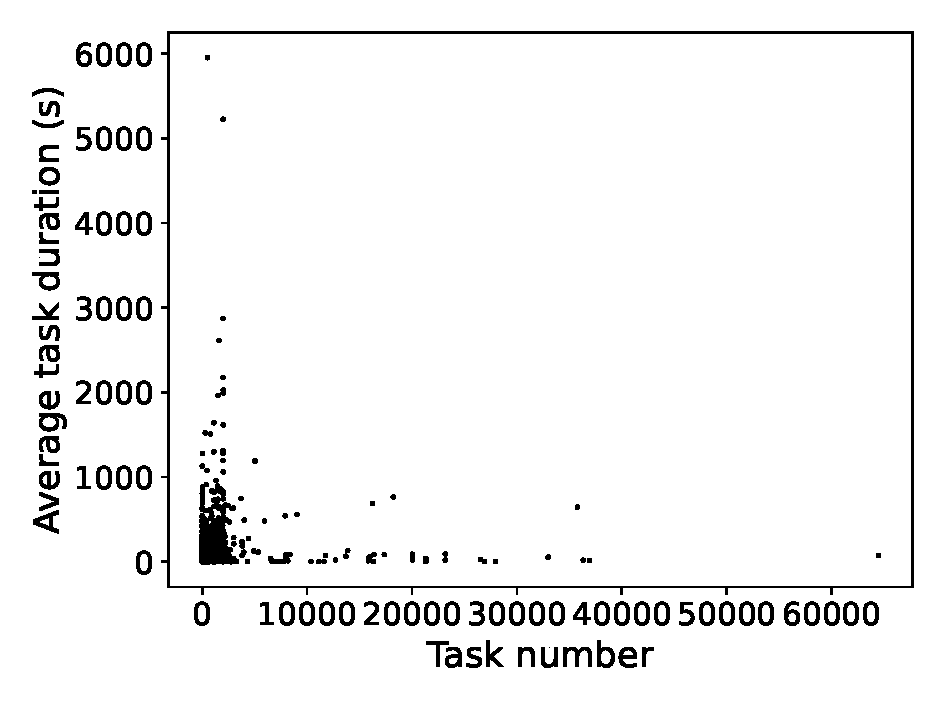
\includegraphics[width=0.47\linewidth]{Image2/JobDistribution_Ali20172D.eps}%
%\label{fig_second_case}
%\label{Fg:eg1}
}
\hfil
\subfloat[Alibaba 2018]
%
{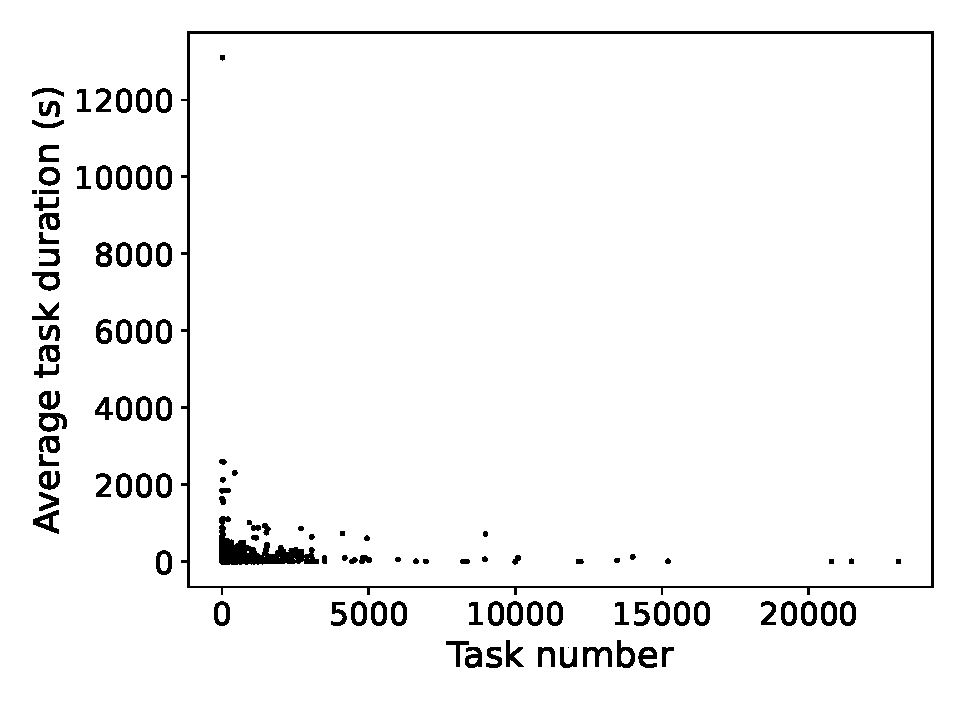
\includegraphics[width=0.48\linewidth]{Image2/JobDistribution_Ali2018_total2D.eps}%
%\label{Fg:eg2}
}
\caption{Job characteristic distribution of two datasets}
\label{fig:distribution2}
\end{figure}

We use cluster job traces sourced from the Alibaba Cluster Trace Program \cite{Ali2017}, which contains cluster traces of different years from real production. We pre-process the raw trace files of years 2017 and 2018, extract the key information including the arrival time, task number, average memory consumption and task processing times of each job. A continuous sequence of 10,000 jobs is randomly selected from each trace to serve as the dataset driving our simulations. The job characteristics of selected sequences are shown in Fig. \ref{fig:distribution} and Fig. \ref{fig:distribution_data}. 
Both sequences exhibit a heavy-tailed distribution, in which a small subset of jobs accounts for a disproportionately large share of the total computation load. We take the average memory consumption of each job as its data partition size. The average memory consumption records in the data traces are normalized values with respect to the memory capacity of the servers in the cluster. We derive the exact data partition size assuming that each server has 128GB RAM, under which the largest data partition is about 4GB. The average task number per job, average task processing time and average data partition size of all jobs are shown in Table \ref{tab:average_characteristic}.

%We use cluster job traces from Alibaba \cite{Ali2017} and Google \cite{Gg2019}. The Alibaba trace is sourced from the Alibaba Cluster Trace Program \cite{Ali2017}, and contains information on approximately 16 million tasks collected from 1300 machines over a period of 12 hours in August 2017. The Google trace is derived from the Borg cluster workload traces\cite{Gg2019}, containing around 30 GB compressed data of task events (e.g., a task is scheduled, completed or aborted) from Google's eight Borg cells over the month of May 2019. We pre-process both raw traces to extract key information, including the arrival time, task count, data partition size and task duration of each job. From each trace, a continuous sequence of 10,000 jobs is randomly selected to serve as the dataset driving our simulations. Characteristics of both datasets are shown in Fig. \ref{fig:distribution} and Fig. \ref{fig:distribution_data}. Both datasets exhibit a heavy-tailed distribution, in which a small subset of jobs accounts for a disproportionately large share of the total workload.  The data partition record in both data traces is a normalized value in homogeneous clusters; We derive the exact partition size with assumption that each cluster has 128GB RAM. The average task duration, average task count and average data partition size is shown in Table \ref{tab:average_characteristic}.


\begin{figure}[t]
\centering
\subfloat[Alibaba 2017]
{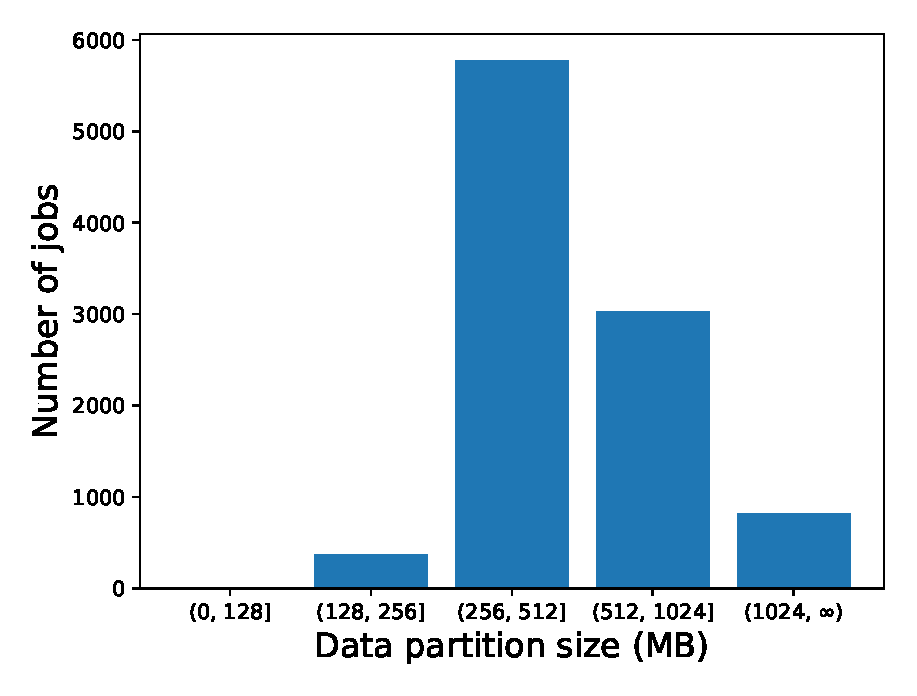
\includegraphics[width=0.455\linewidth]{Image2/data_Distribution_Ali2017.eps}%
%\label{fig_second_case}
%\label{Fg:eg1}
}
\hfil
\subfloat[Alibaba 2018]
%
{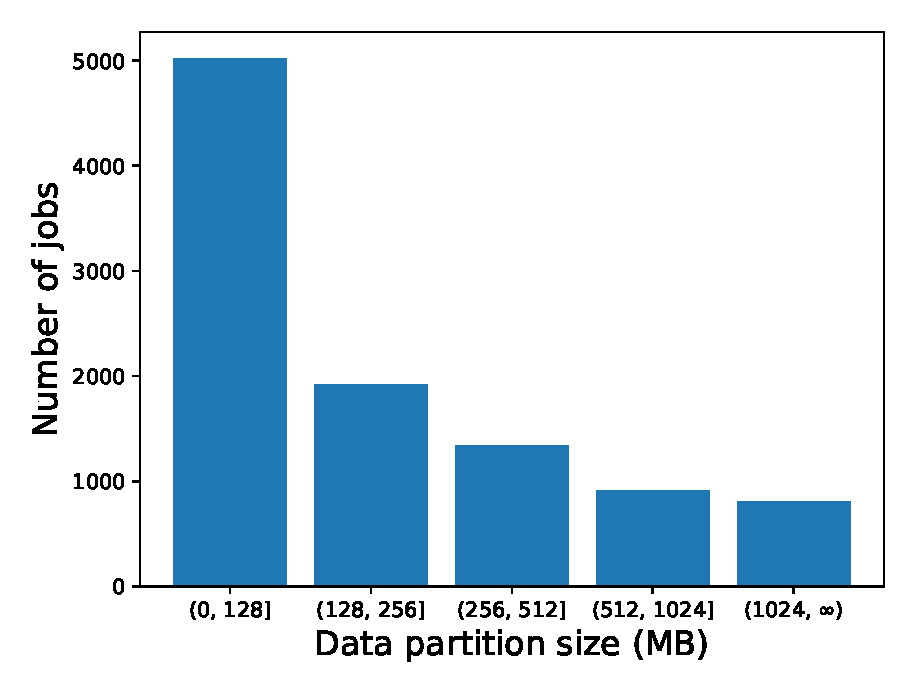
\includegraphics[width=0.455\linewidth]{Image2/data_Distribution_Ali2018_total.eps}%
%\label{Fg:eg2}
}
\caption{Data partition size distribution of two datasets}
\label{fig:distribution_data}
\end{figure}

\begin{table}[t]
\centering
\begin{tabular}{@{}lll@{}}
\hline
Characteristics & Alibaba 2017 & Alibaba 2018 \\
\hline
Average task number per job & $266.01$ & $94.70$ \\
\hline
Average task processing time (s) & $129.14$ & $82.41$ \\
\hline
Average data partition size (MB) & $661.15$ & $453.31$ \\
\hline
\end{tabular}
\caption{Job characteristics of two datasets}
\label{tab:average_characteristic}
\end{table}

\begin{figure*}[t]
\centering
\subfloat[utilization = 50\%]
{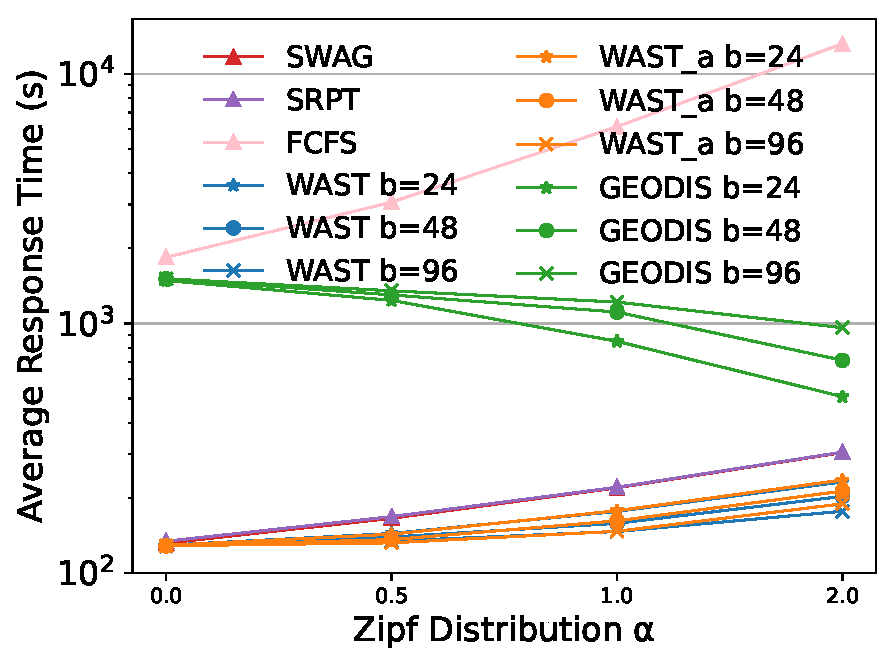
\includegraphics[width=0.24\textwidth]{Image2/Workload_Ali2018_4_50_GEODIS.eps}%
%\label{fig_second_case}
%\label{Fg:eg1}
}
\hfil
\subfloat[utilization = 60\%]
%
{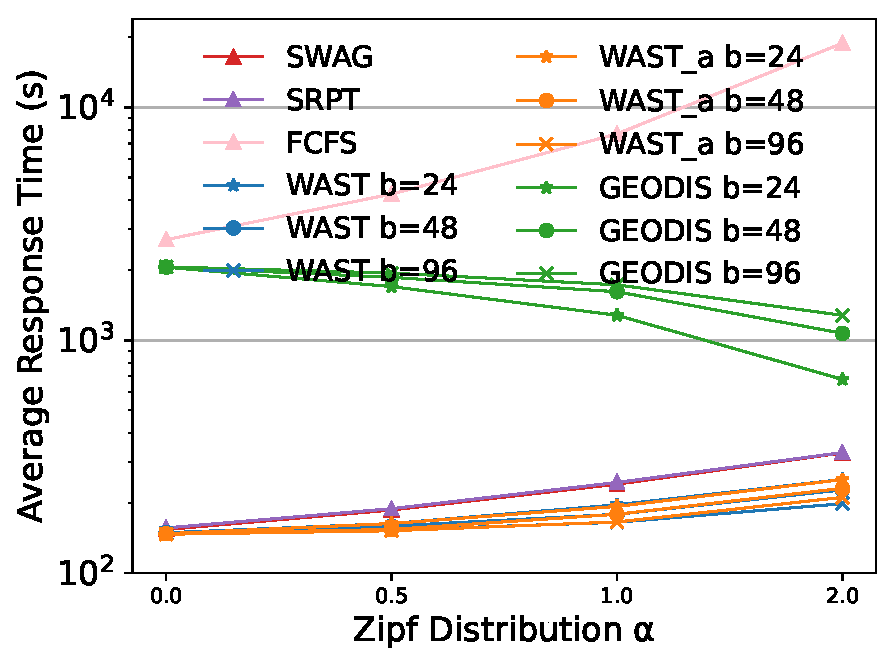
\includegraphics[width=0.24\textwidth]{Image2/Workload_Ali2018_4_60_GEODIS.eps}%
%\label{Fg:eg2}
}
\hfil
\subfloat[utilization = 70\%]
%
{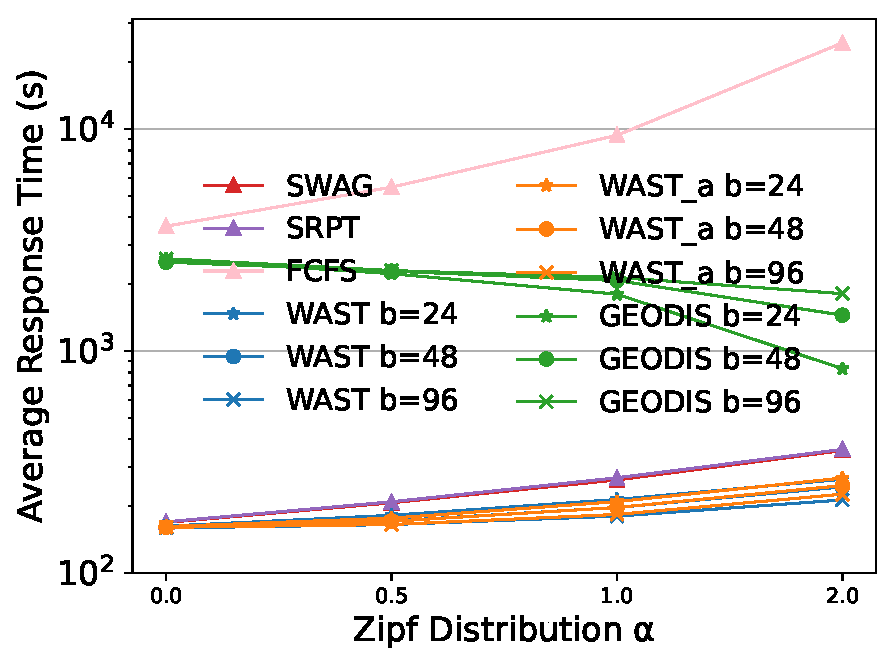
\includegraphics[width=0.24\textwidth]{Image2/Workload_Ali2018_4_70_GEODIS.eps}%
%\label{Fg:eg2}
}
\hfil
\subfloat[utilization = 80\%]
%
{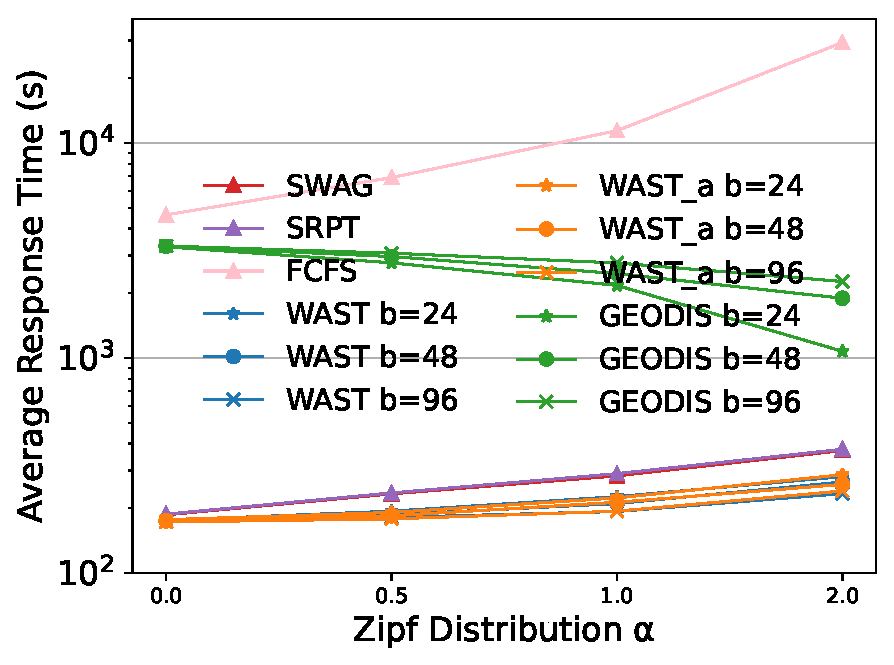
\includegraphics[width=0.24\textwidth]{Image2/Workload_Ali2018_4_80_GEODIS.eps}%
%\label{Fg:eg2}
}
\caption{Average Job Response Time Compared with GEODIS, Alibaba 2018}
\label{fig:JRT_GEODIS}
\end{figure*}

\begin{figure*}[t]
\centering
\subfloat[utilization = 50\%]
{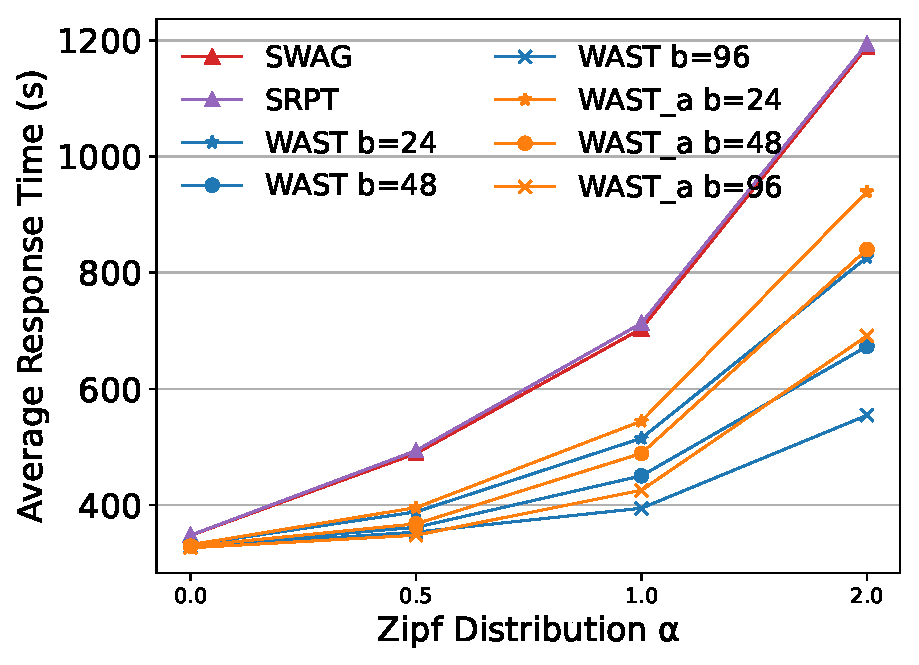
\includegraphics[width=0.24\textwidth]{Image2/Workload_Ali2017_50.eps}%
%\label{fig_second_case}
%\label{Fg:eg1}
}
\hfil
\subfloat[utilization = 60\%]
%
{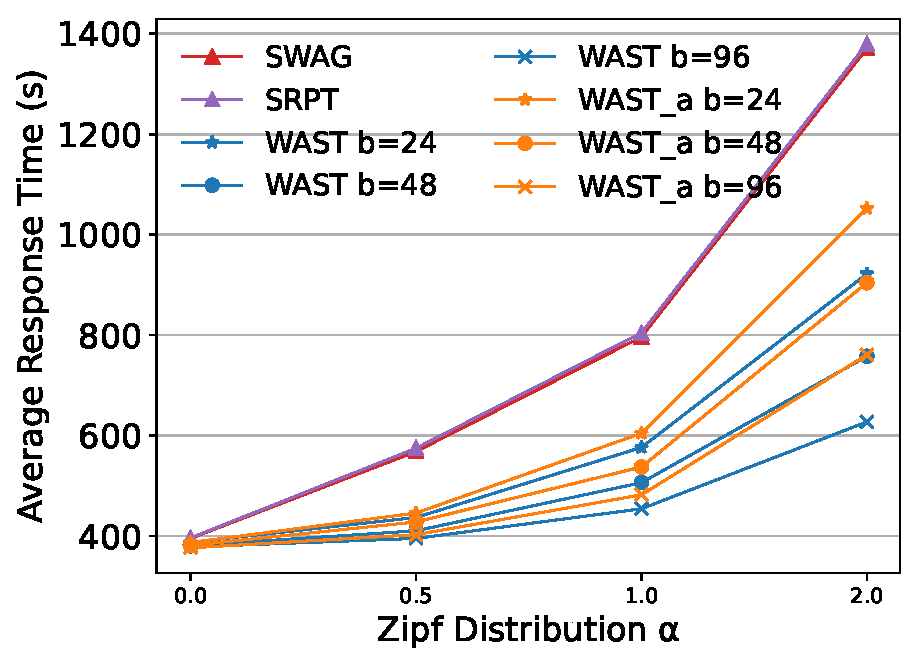
\includegraphics[width=0.24\textwidth]{Image2/Workload_Ali2017_60.eps}%
%\label{Fg:eg2}
}
\hfil
\subfloat[utilization = 70\%]
%
{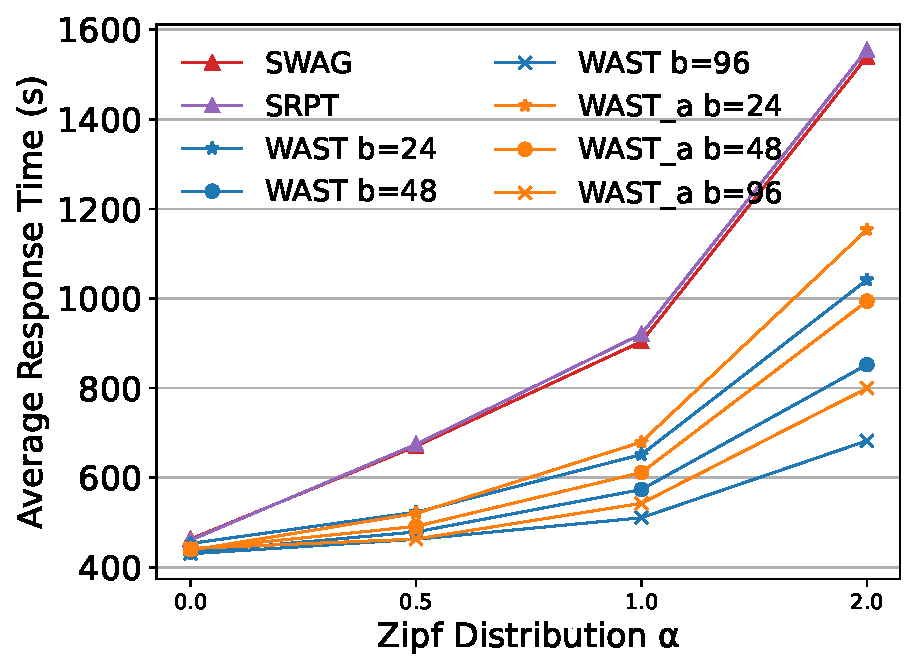
\includegraphics[width=0.24\textwidth]{Image2/Workload_Ali2017_70.eps}%
%\label{Fg:eg2}
}
\hfil
\subfloat[utilization = 80\%]
%
{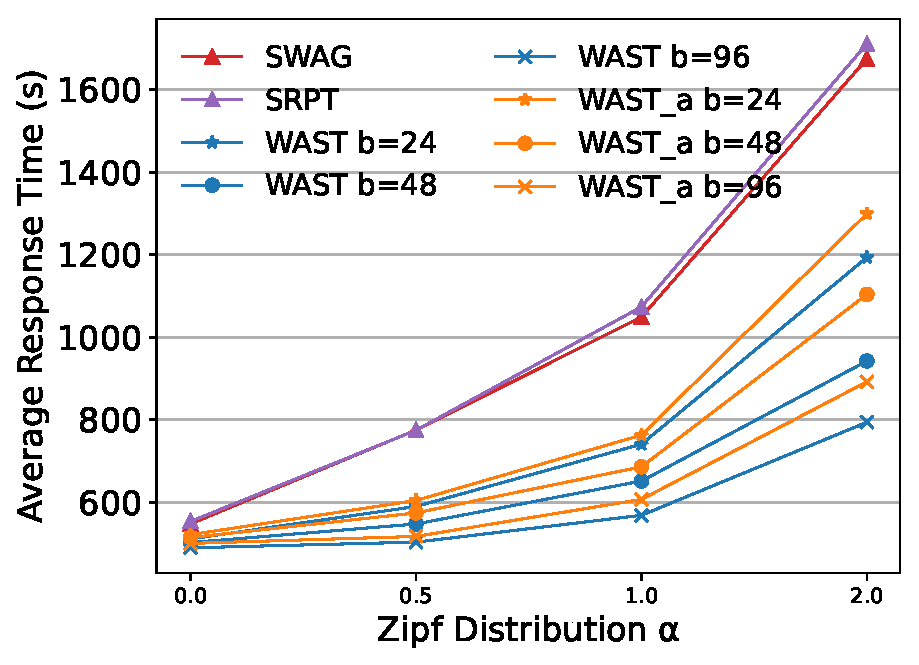
\includegraphics[width=0.24\textwidth]{Image2/Workload_Ali2017_80.eps}%
%\label{Fg:eg2}
}
\caption{Average Job Response Time, Alibaba 2017}
\label{fig:JRT}
\end{figure*}

\begin{figure*}[t]
\centering
\subfloat[utilization = 50\%]
{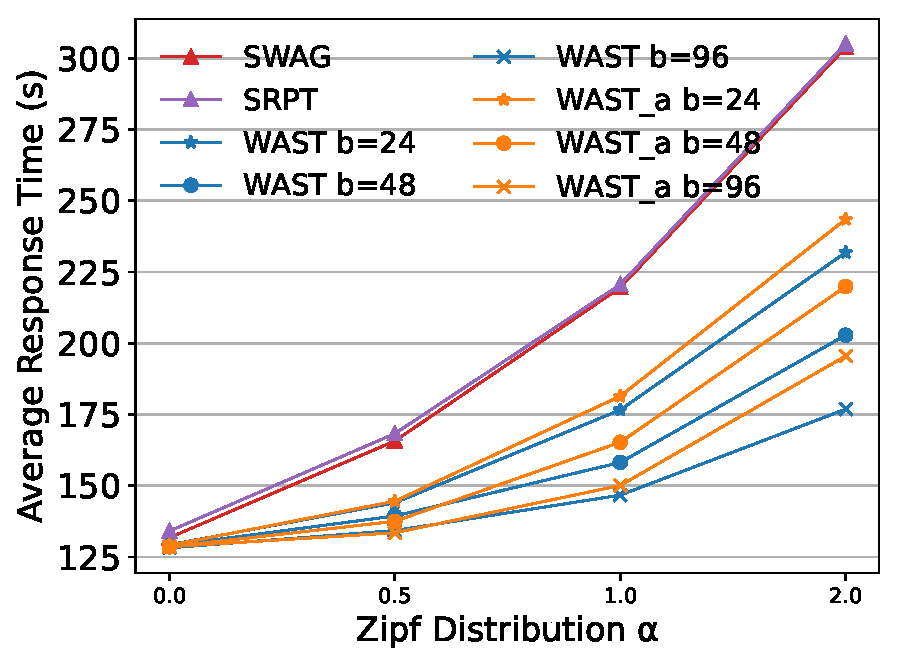
\includegraphics[width=0.24\textwidth]{Image2/Workload_Ali2018_4_50.eps}%
%\label{fig_second_case}
%\label{Fg:eg1}
}
\hfil
\subfloat[utilization = 60\%]
%
{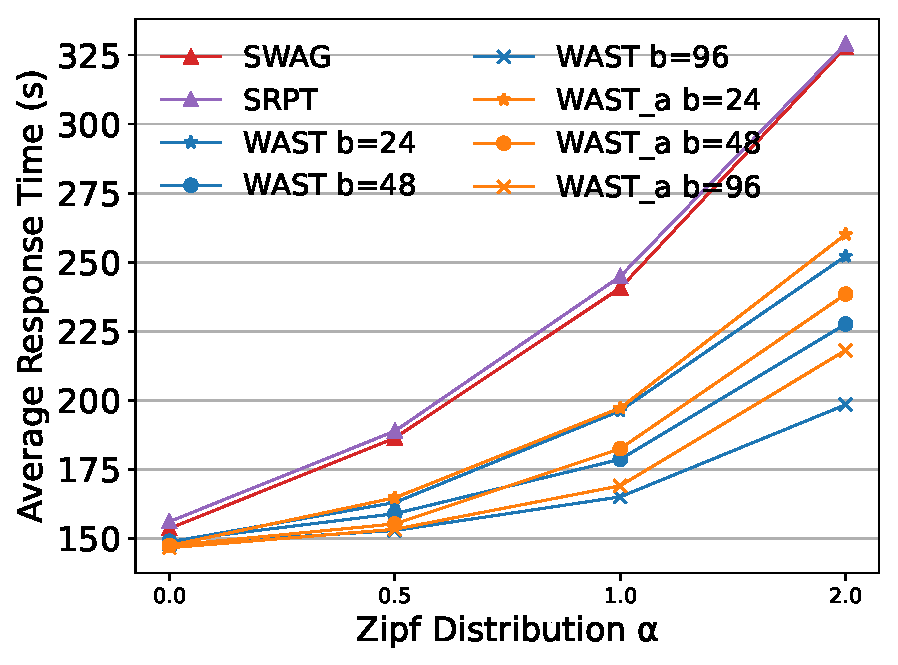
\includegraphics[width=0.24\textwidth]{Image2/Workload_Ali2018_4_60.eps}%
%\label{Fg:eg2}
}
\hfil
\subfloat[utilization = 70\%]
%
{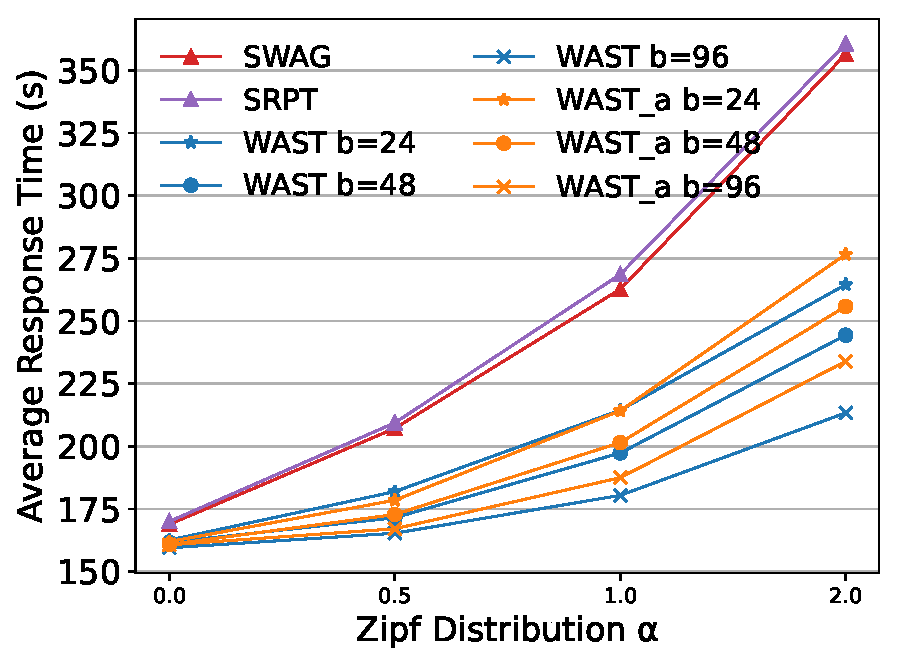
\includegraphics[width=0.24\textwidth]{Image2/Workload_Ali2018_4_70.eps}%
%\label{Fg:eg2}
}
\hfil
\subfloat[utilization = 80\%]
%
{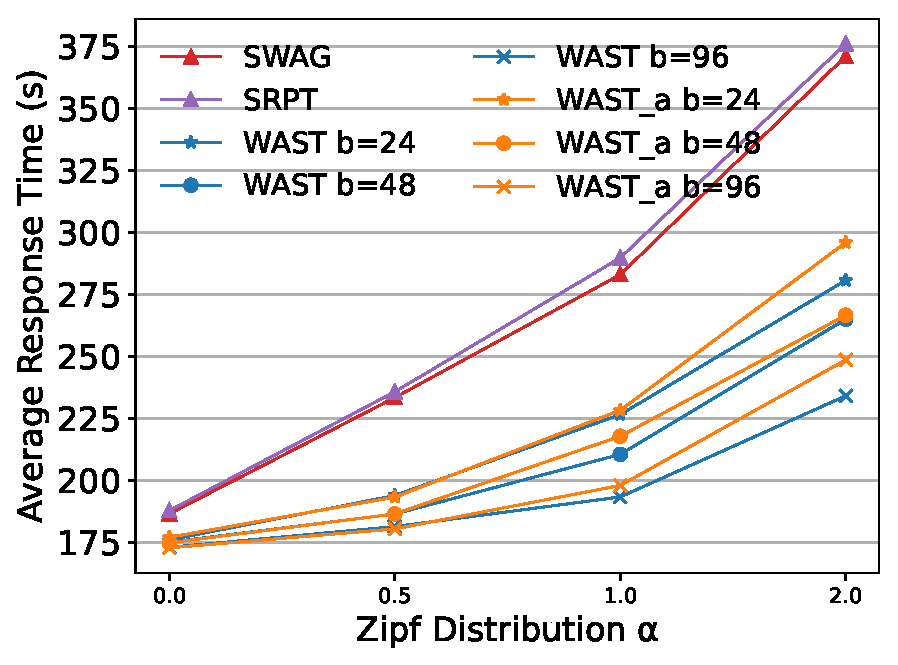
\includegraphics[width=0.24\textwidth]{Image2/Workload_Ali2018_4_80.eps}%
%\label{Fg:eg2}
}
\caption{Average Job Response Time, Alibaba 2018}
\label{fig:JRT2}
\end{figure*}


\subsection{System Configuration}
We simulate a distributed system of $m$ sites, each with the same number of computing slots. Each task is assumed to take up one computing slot to run and release it after completion. Due to the switching overhead consideration, we assume that the system does not allow preemption during task execution. For each job, the initial distribution of its tasks among the sites is generated by a Zipf distribution: the numbers of tasks placed at the $m$ sites are proportional to $1, \frac{1}{2^\alpha}, \frac{1}{3^\alpha}, ..., \frac{1}{m^\alpha}$, where $\alpha$ is a Zipf parameter. A higher $\alpha$ implies a more skewed distribution (a higher proportion of tasks are concentrated at fewer sites), whereas $\alpha$ = $0$ indicates a uniform distribution. In the experiments, we test four Zipf distributions with $\alpha$ set to $0$, $0.5$, $1$ and $2$ to simulate different task distributions of jobs. After the task distribution is generated, we shuffle the order of the sites when deploying each job's task distribution, so that the total workload at each site 
%(i.e., the total execution time of the tasks of all jobs deployed at each site) 
is roughly balanced. 
We scale the arrival times of the jobs in the datasets to simulate different levels of overall system utilization. We assume that the system is fully connected, i.e., a direct link exists between any two sites. The available bandwidth is set to $24$Mbps, $48$Mbps or $96$Mbps for all links. We experiment with different numbers of sites, different numbers of computing slots per site, and different levels of system utilization. The results show similar performance trends. Due to space limitations, we focus on presenting the results for $m=10$ sites, 32 computing slots per site, and system utilization = $50\%$, $60\%$, $70\%$ and $80\%$.  
%\sout{and a system workload of 60\%}
%As mentioned in Section \ref{sec:dataset}, the average data partition size of the Alibaba and Google data trace is a normalized value; We suppose that 

\subsection{Scheduling Policies}
In Section \ref{sec:WAST}, we have introduced the WAST algorithm and its fast approximation WAST\_a. For comparison, we also simulate the following baseline algorithms.
\begin{itemize}
    \item \textbf{First-Come-First-Serve (FCFS)}: FCFS simply schedules jobs in the order of their arrival times. When a computing slot becomes available, it is assigned to the job that arrives the earliest and has pending tasks.
    
    \item \textbf{Shortest Remaining Processing Time (SRPT)}: SRPT schedules jobs based on their estimated completion times in the case that each job runs alone in the system. More specifically, it estimates the completion time of a job $J_k$ as $\max_{j \in[m]} \lceil d_{kj}/u_j\rceil \cdot l_k$, and executes pending jobs based on this estimation from low to high.% The original SRPT assumes that each site has one computation slot only (i.e., the estimated completion time of each job $J_k$ is equal to the $\max_{j \in[m]} (l_k*d_{kj})$), and we adapt it to the case that each site has multiple slots. %In other words, SRPT places each job's distributed workload to the empty system and computes its job response time, and the job execution order is derived based on these estimated job response times.

    \item \textbf{Workload-Aware Greedy Scheduling (SWAG)} \cite{hung2015scheduling}: SWAG greedily schedules jobs iteratively by estimating their completion times based on scheduled workloads without using network resources to transfer tasks between sites. %It iteratively selects the job with the lowest completion time and add the job's computation loads to the system. 
    Our WAST algorithm degenerates to SWAG when network resources are not available in the system. %In each round, given the computation load of scheduled jobs of previous rounds, SWAG traverses each unscheduled job and computes its estimated completion time by assigning its task to the corresponding sites%SWAG is also designed for the single-slot case and it does not consider utilizing the network resource within the system. We modify SWAG to support the case where each site has multiple computation slots.

    \item \textbf{GEODIS} \cite{GEODIS}: GEODIS models job scheduling in geo-distributed data centers as a joint optimization of task placement and data access. It employs a heuristic scheduling algorithm which is triggered when any data center completes its scheduled workload. The objective of scheduling is to minimize the makespan of job execution (the latest job completion time) by selectively migrating data over faster network links when local servers are overloaded.
\end{itemize}
%
%The improvement becomes more pronounced when jobs' workload distribution is more skewed among sites and when higher bandwidth is available, since the utilization of network resource has greater potential in mitigating the workload imbalances of each job under these conditions. Furthermore, the algorithm performs better on the Alibaba 2017 data trace
In the experiments, we use OR-Tools \cite{ortools} to solve the minimum-cost flow problems in WAST. All algorithms (except FCFS) take the average task processing time of each job as input for scheduling and assume that the processing times of all tasks of the job are equal to the average. The simulation, on the other hand, uses the real processing times of individual tasks recorded in the trace to derive the job response time.

\subsection{Experimental Results}
Fig. \ref{fig:JRT_GEODIS} shows the performance of all algorithms in terms of average job response time. Due to space limitations, we only present the results for the Alibaba 2018 dataset 
%under system utilization of $60\%$ and $80\%$ 
(the results for the Alibaba 2017 dataset are similar). Note that the y-axis is plotted on a logarithmic scale. The results indicate that the average job response times of FCFS and GEODIS are one to two orders of magnitude higher than the other algorithms. This is because FCFS does not optimize job execution order and GEODIS is primarily designed to minimize the makespan.

Figs. \ref{fig:JRT} and \ref{fig:JRT2} zoom into the performance of the remaining algorithms for both datasets. %The results of the FCFS strategy are more than two orders of magnitude higher than those of the other algorithms and hence are not included in the figures. 
Compared to SRPT and SWAG, the average job response time of WAST and WAST\_a is reduced by up to $53.3\%$ for the Alibaba 2017 trace and $42.1\%$ for the Alibaba 2018 trace. The improvement becomes more pronounced when the task distribution of jobs across sites is more skewed and when higher bandwidth is available, as more network resources can be effectively utilized to mitigate the imbalance in the task distribution of jobs under these conditions. Moreover, our WAST algorithm performs better for the Alibaba 2017 trace than the Alibaba 2018 trace. This is because the higher average task number per job in Alibaba 2017 leads to more tasks accumulated at some particular sites under highly uneven task distributions, resulting in increased response times if task transmission is not conducted. This, in turn, allows the WAST algorithm to offload more tasks from peak-load sites, enhancing the advantage of WAST. 
In addition, Figs. \ref{fig:JRT} and \ref{fig:JRT2} show that although WAST\_a compromises the quality of scheduling and performs slightly worse than WAST, it still significantly outperforms the baseline algorithms.%demonstrating that it is an effective approximation to WAST.%the ratio of average task duration to average data partition size is higher in 2017. This allows a greater number of tasks to be transmitted within the average task execution time, thereby providing additional opportunities to reduce job response time through task migration. Furthermore, 

% \begin{figure}[t]
% \centering
% \subfloat[utilization=60\%]
% {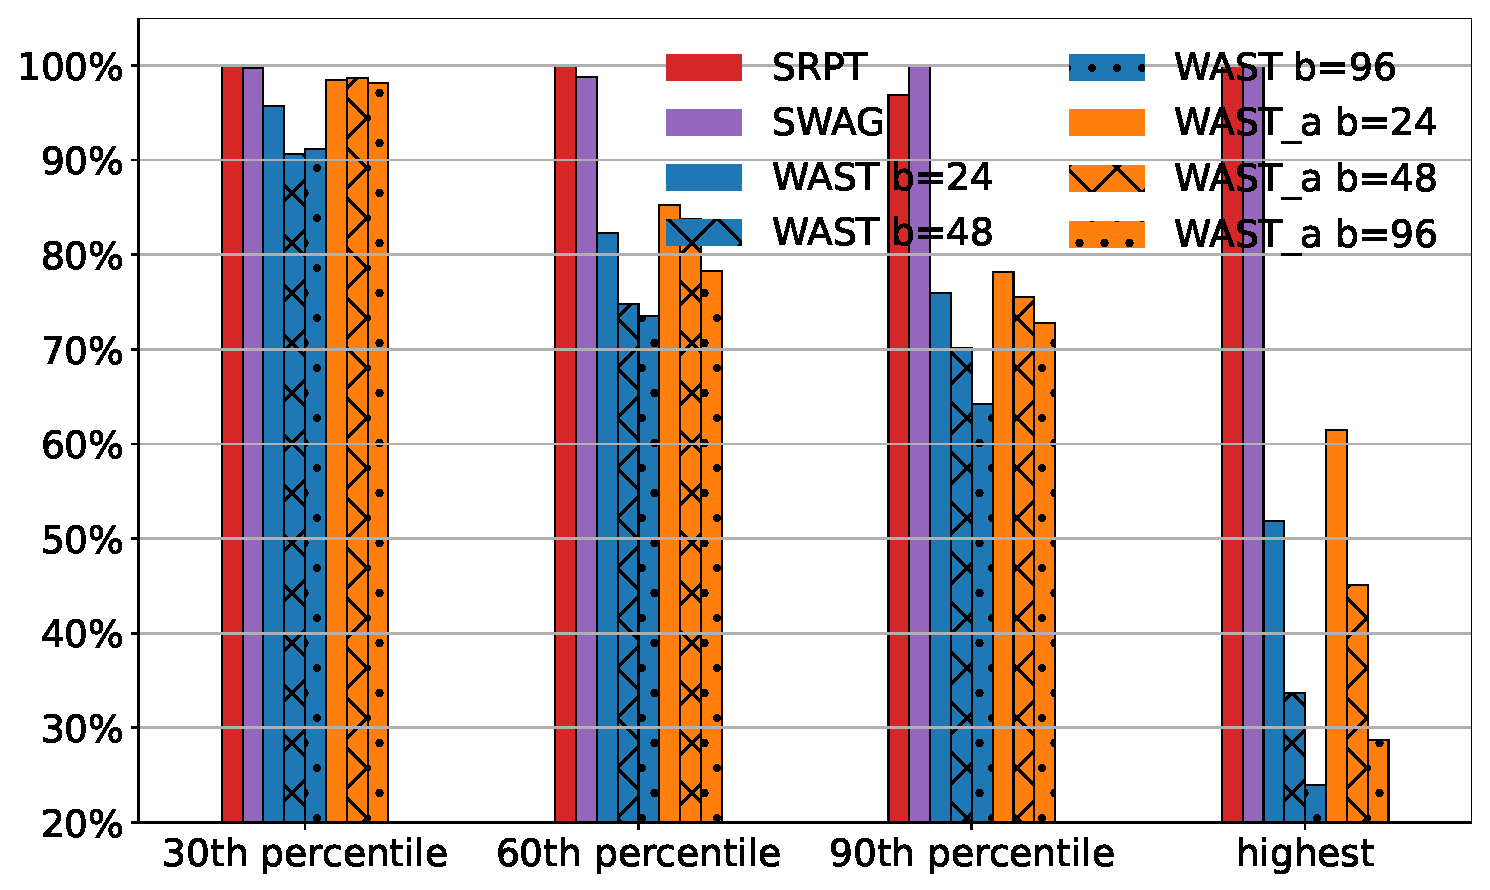
\includegraphics[width=0.48\linewidth]{Image2/CDFpercentile_Ali2017_60.eps}%
% %\label{fig_second_case}
% %\label{Fg:eg1}
% }
% \hfil
% \subfloat[utilization=80\%]
% %
% {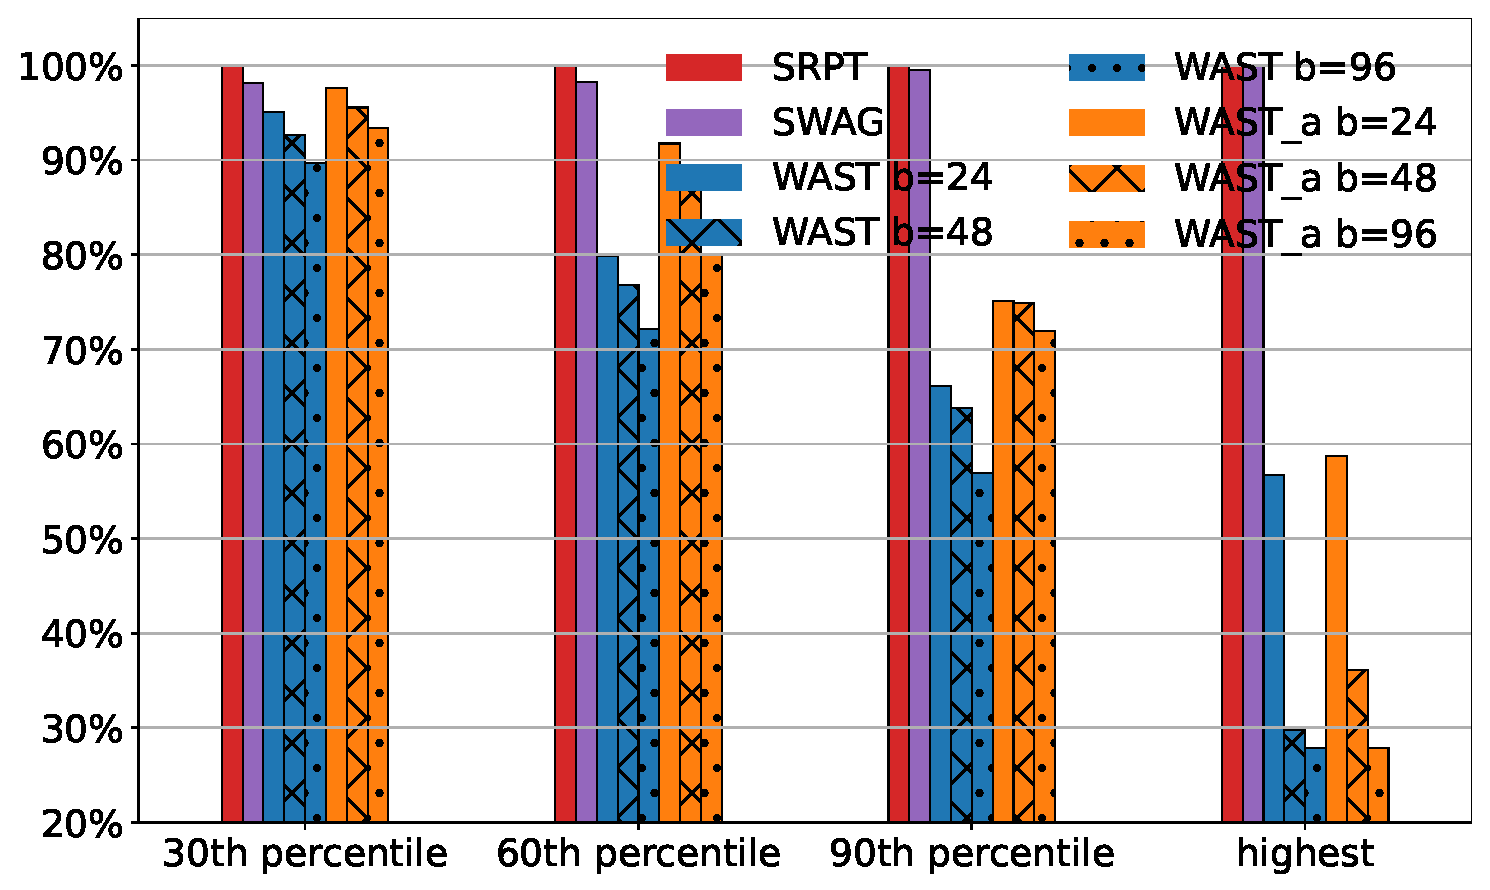
\includegraphics[width=0.48\linewidth]{Image2/CDFpercentile_Ali2017_80.eps}%
% %\label{Fg:eg2}
% }
% \caption{Response Time at Different Percentiles, Alibaba 2017, $\alpha=1$}
% \label{fig:JRT_CDF_2017}
% \end{figure}

% \begin{figure}[t]
% \centering
% \subfloat[utilization=60\%]
% {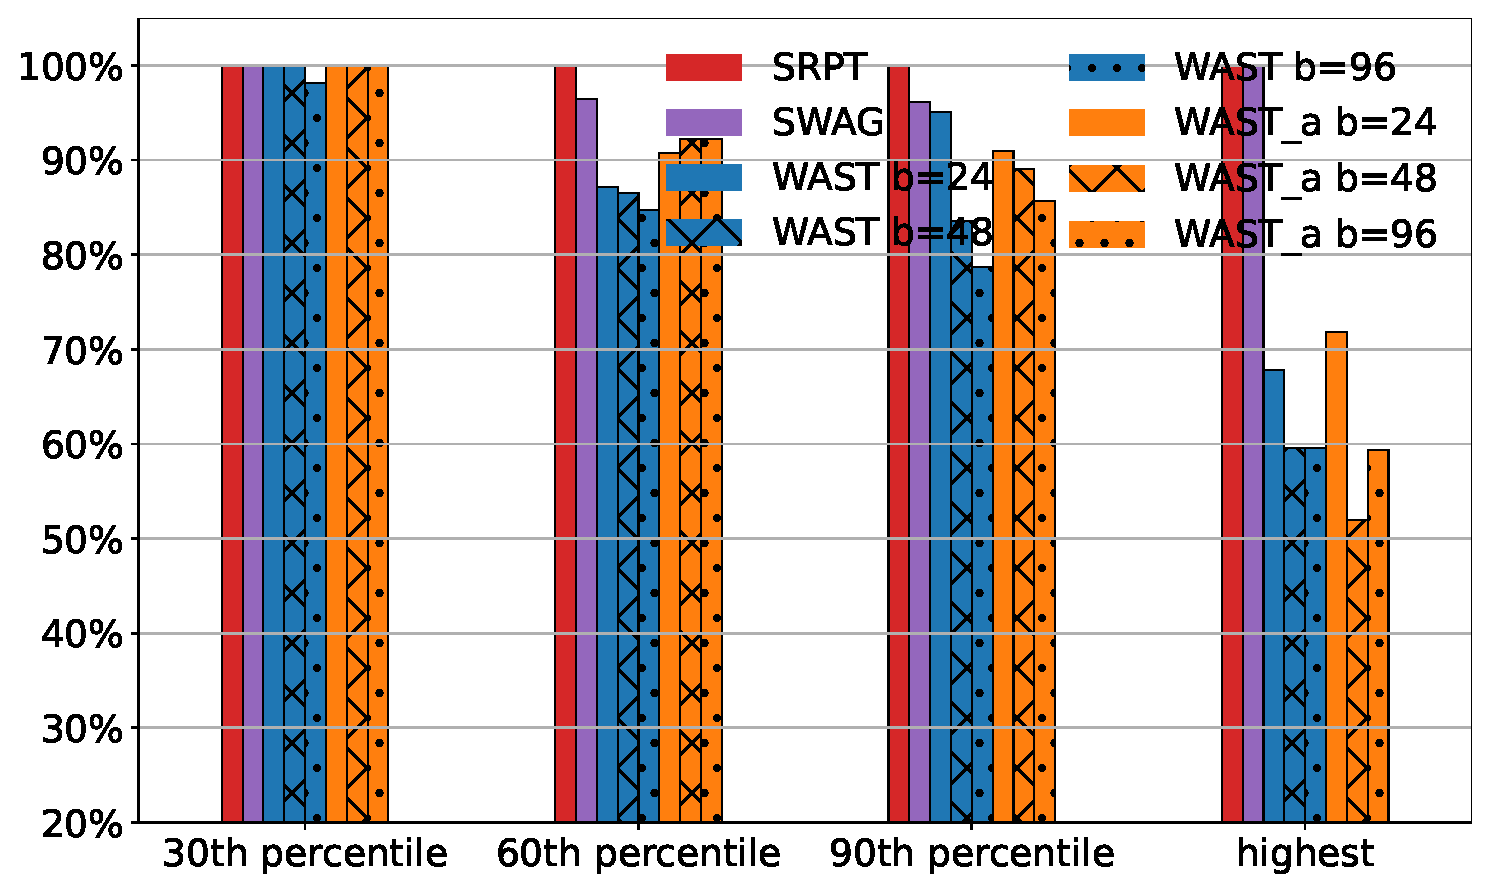
\includegraphics[width=0.48\linewidth]{Image2/CDFpercentile_Ali2018_4_60.eps}%
% %\label{fig_second_case}
% %\label{Fg:eg1}
% }
% \hfil
% \subfloat[utilization=80\%]
% %
% {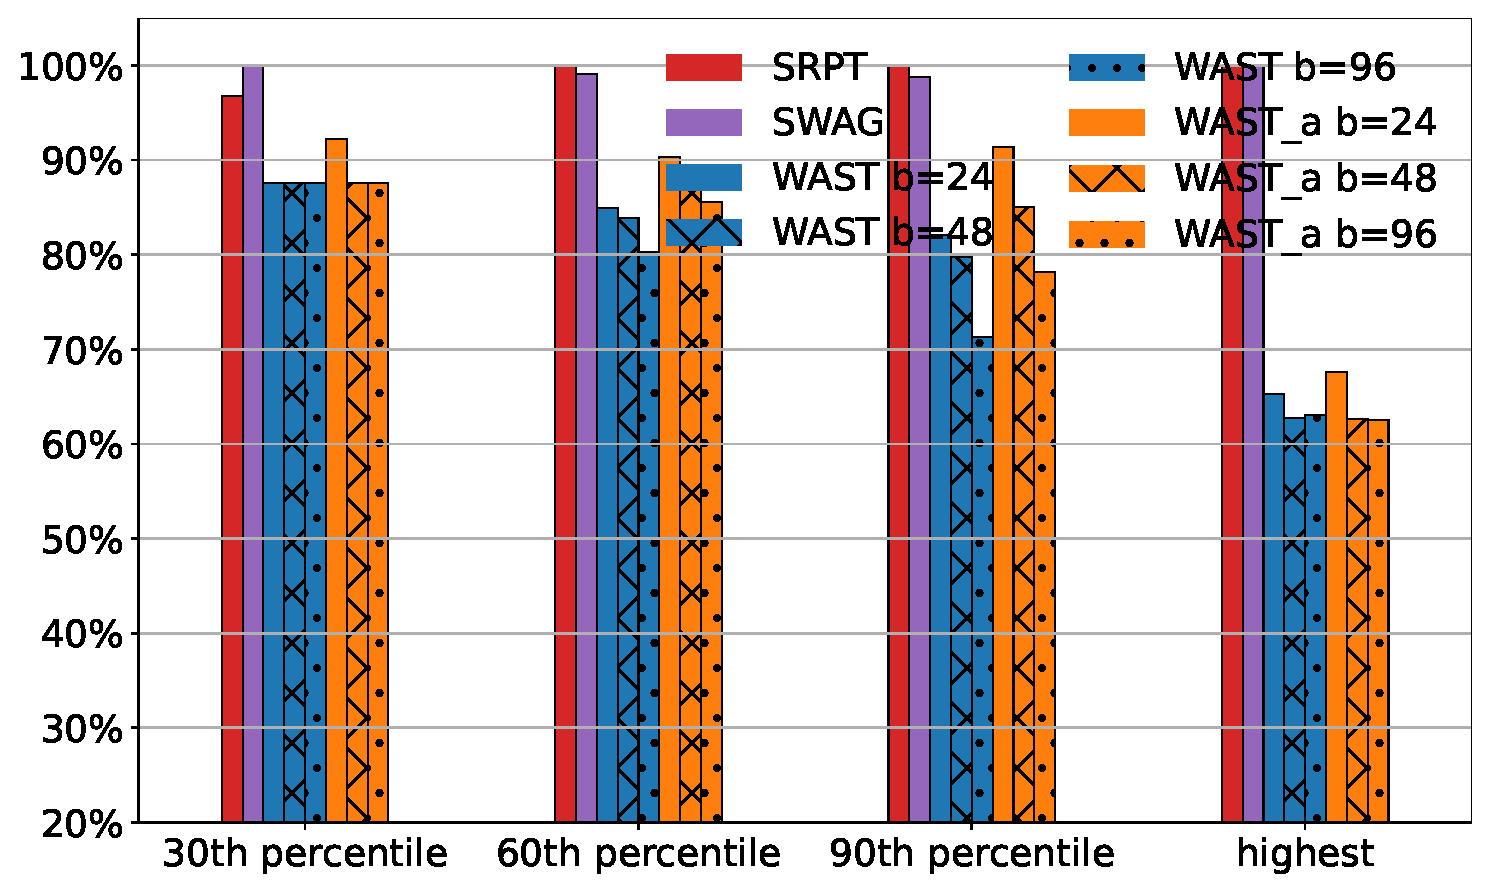
\includegraphics[width=0.48\linewidth]{Image2/CDFpercentile_Ali2018_4_80.eps}%
% %\label{Fg:eg2}
% }
% \caption{Response Time at Different Percentiles, Alibaba 2018, $\alpha=1$}
% \label{fig:JRT_CDF_2018}
% \end{figure}
Figs. \ref{fig:JRT_CDF} and \ref{fig:JRT_CDF2} show the $30$th, $60$th, $90$th percentiles and the highest job response times for both datasets, under the Zipf distribution with $\alpha=1$. For each percentile, the longest job response time among algorithms is normalized to 1, and the job response times of other algorithms are expressed relative to it. It can be seen that jobs in the lower percentiles have little improvement when the WAST and WAST\_a algorithms are applied, since these jobs are small and have already achieved nearly best response times under the SRPT and SWAG strategies which favor small jobs. On the other hand, WAST and WAST\_a can significantly enhance the performance of large jobs whose response times are relatively longer by transferring their tasks to mitigate their imbalanced task distributions. The highest job response time can be improved by more than $70\%$, as shown in Fig. \ref{fig:JRT_CDF}.

\begin{figure*}[t]
\centering
\subfloat[utilization = 50\%]
{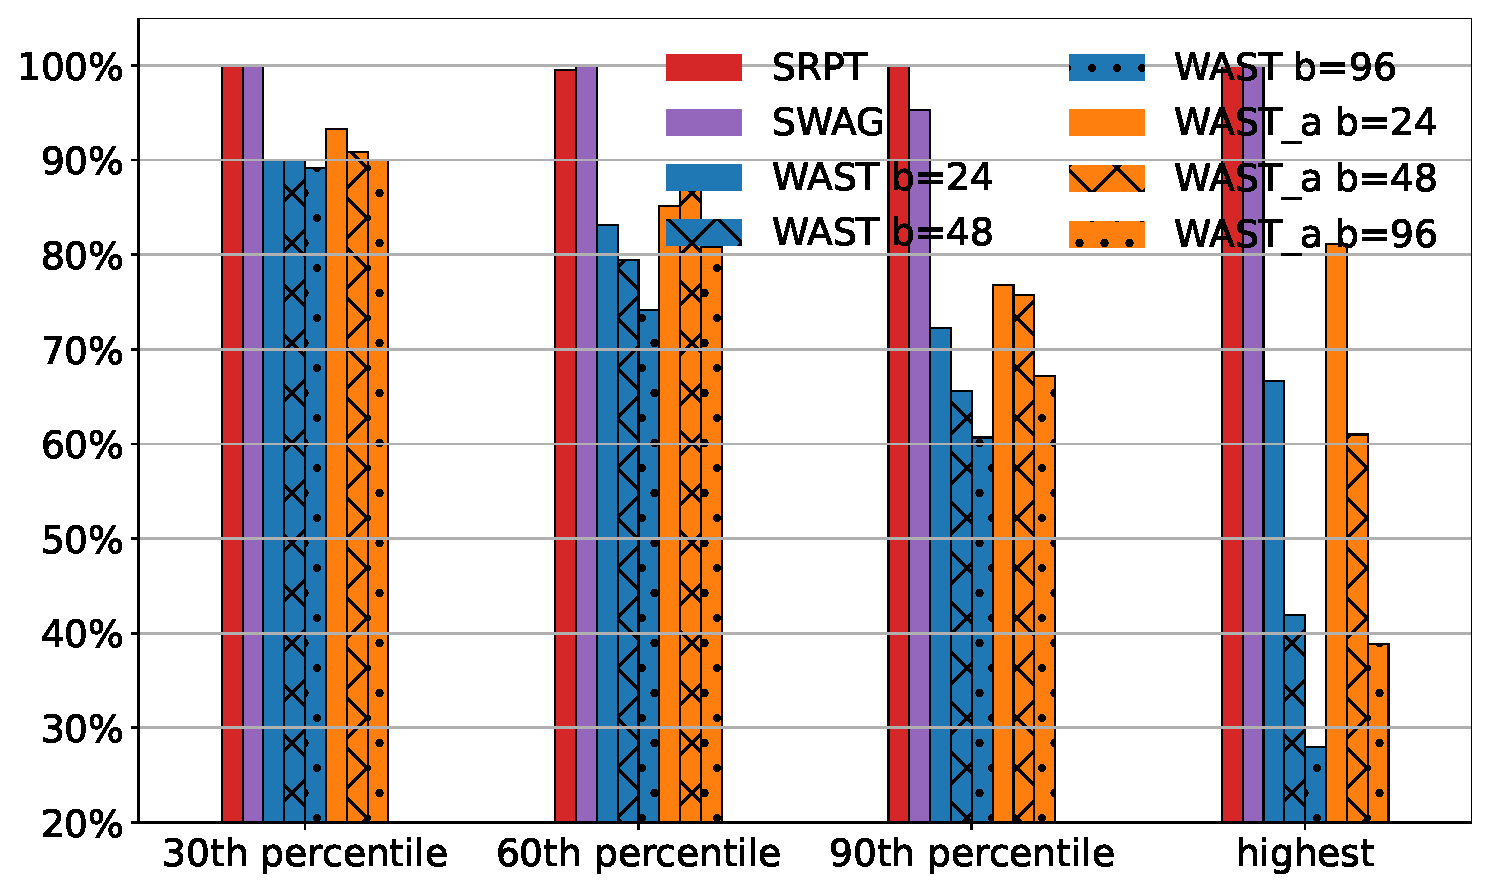
\includegraphics[width=0.24\textwidth]{Image2/CDFpercentile_Ali2017_50.eps}%
\label{fig:JRT_CDF_a}
}
\hfil
\subfloat[utilization = 60\%]
%
{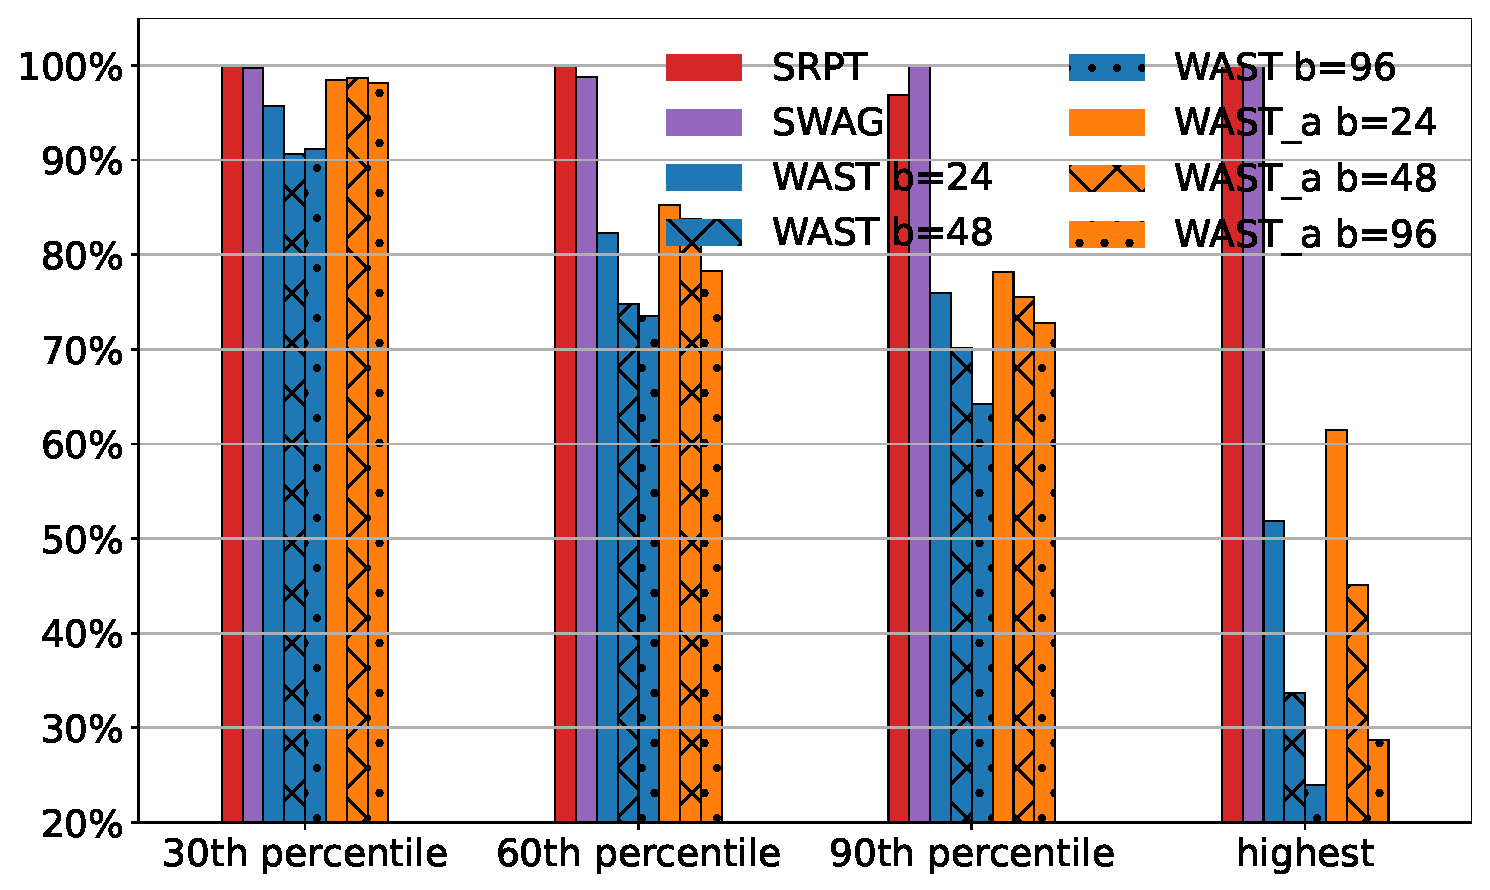
\includegraphics[width=0.24\textwidth]{Image2/CDFpercentile_Ali2017_60.eps}
\label{fig:JRT_CDF_b}
}%
\hfil
\subfloat[utilization = 70\%]
%
{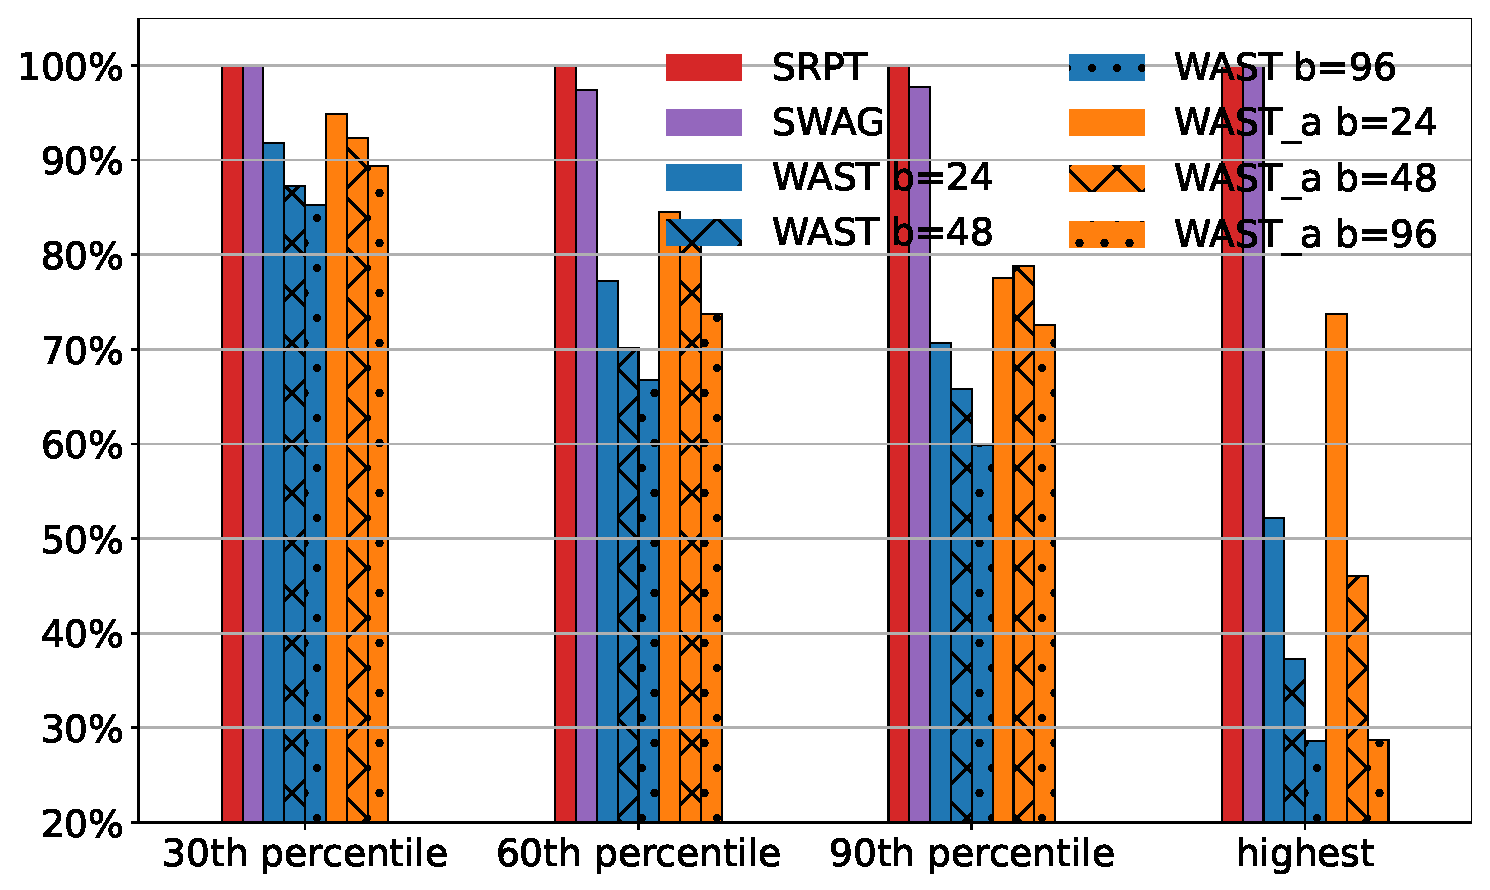
\includegraphics[width=0.24\textwidth]{Image2/CDFpercentile_Ali2017_70.eps}}%
\hfil
\subfloat[utilization = 80\%]
%
{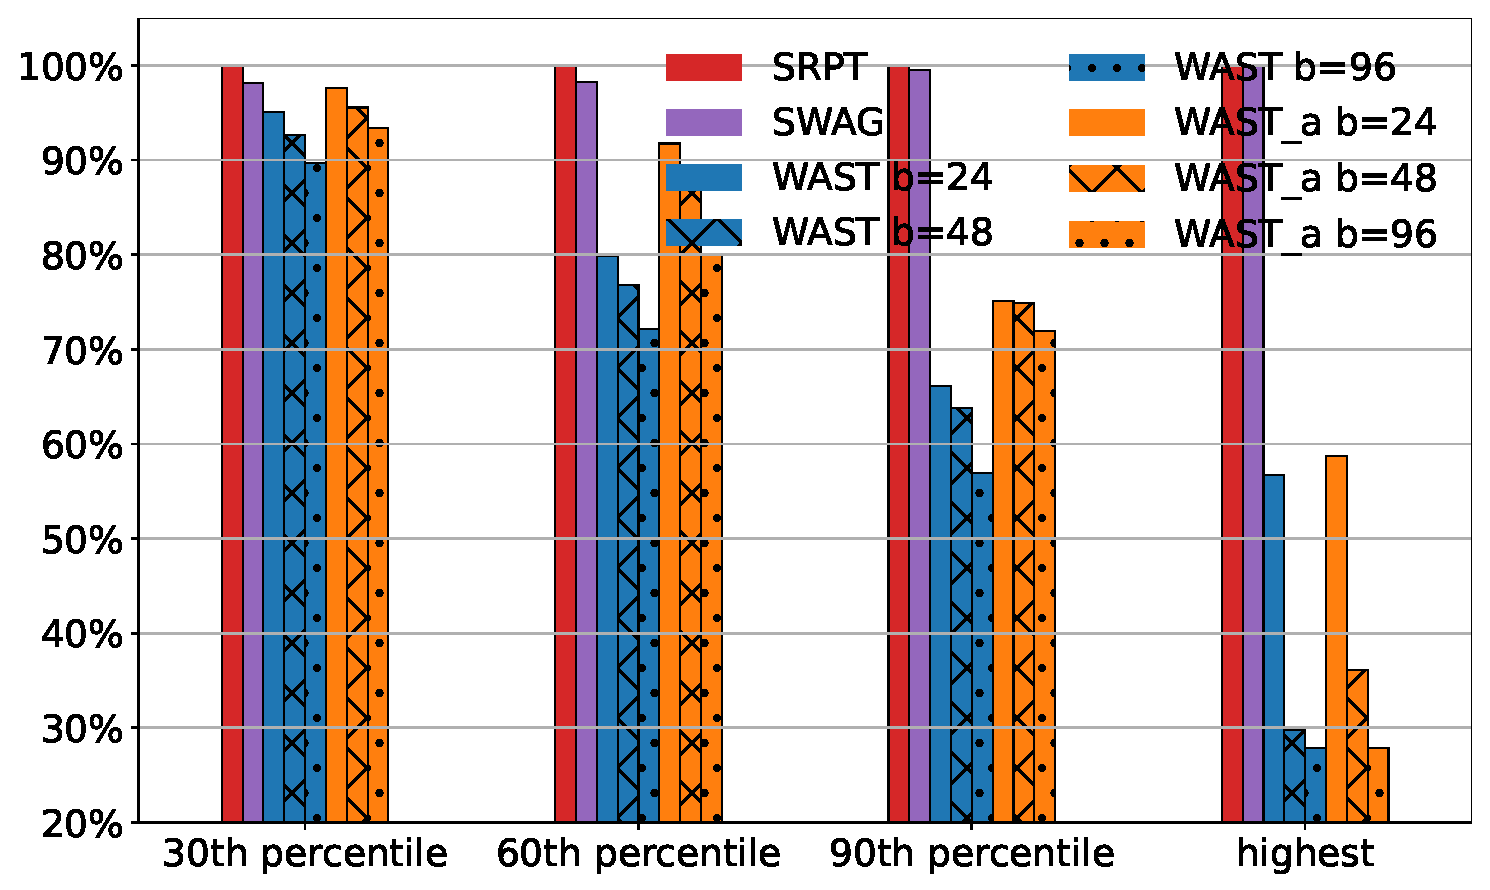
\includegraphics[width=0.24\textwidth]{Image2/CDFpercentile_Ali2017_80.eps}
%\label{Fg:eg2}
}
\caption{Job Response Time at Different Percentiles, Zipf Distribution $\alpha=1$, Alibaba 2017}
\label{fig:JRT_CDF}
\end{figure*}

\begin{figure*}[t]
\centering
\subfloat[utilization = 50\%]
{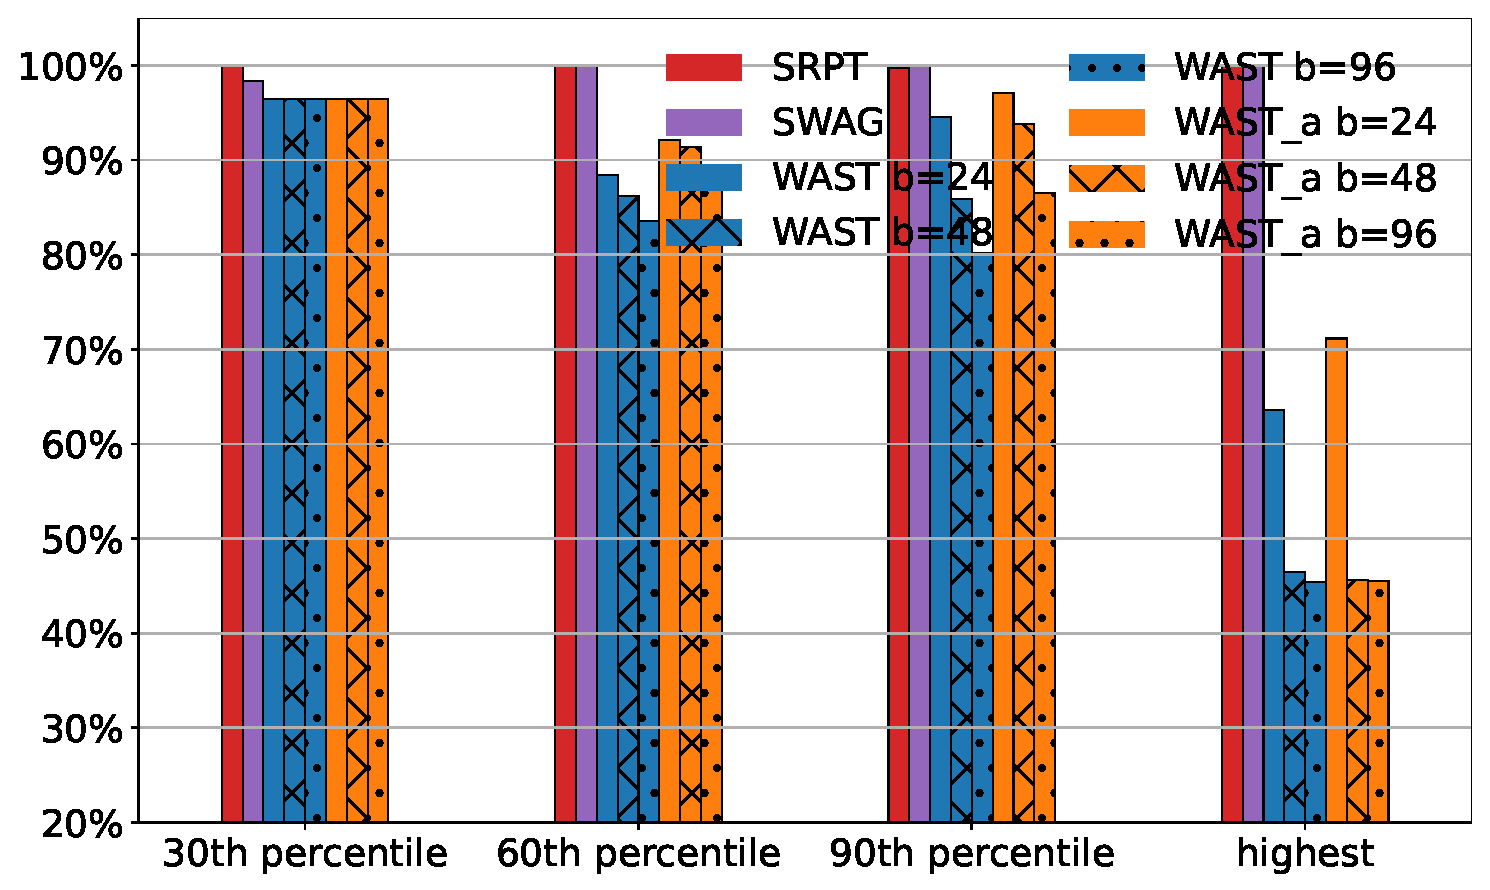
\includegraphics[width=0.24\textwidth]{Image2/CDFpercentile_Ali2018_4_50.eps}%
\label{fig:JRT_CDF_a}
}
\hfil
\subfloat[utilization = 60\%]
%
{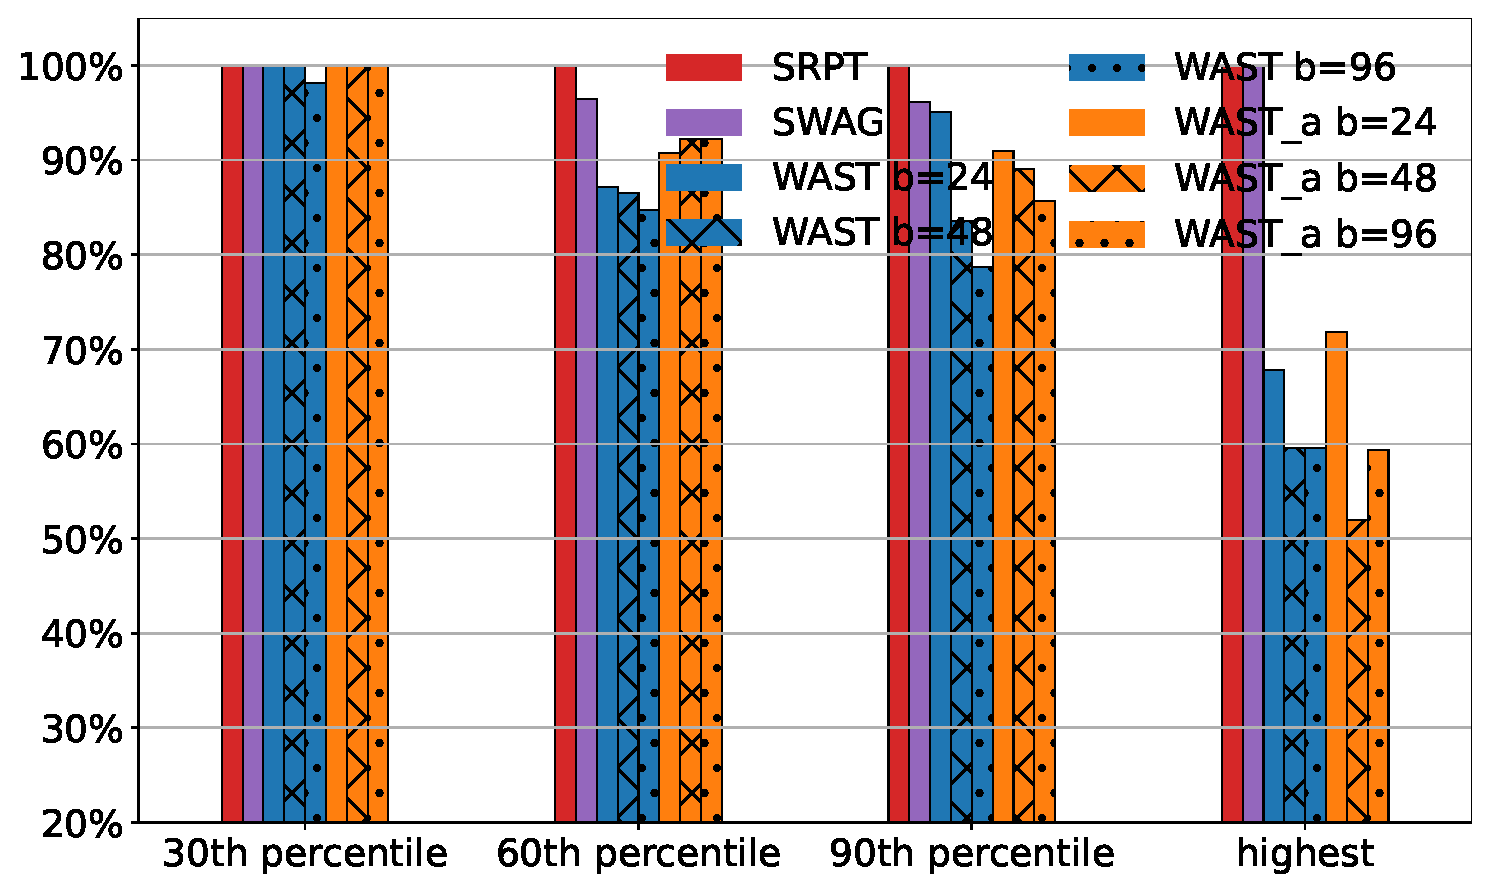
\includegraphics[width=0.24\textwidth]{Image2/CDFpercentile_Ali2018_4_60.eps}
\label{fig:JRT_CDF_b}
}%
\hfil
\subfloat[utilization = 70\%]
%
{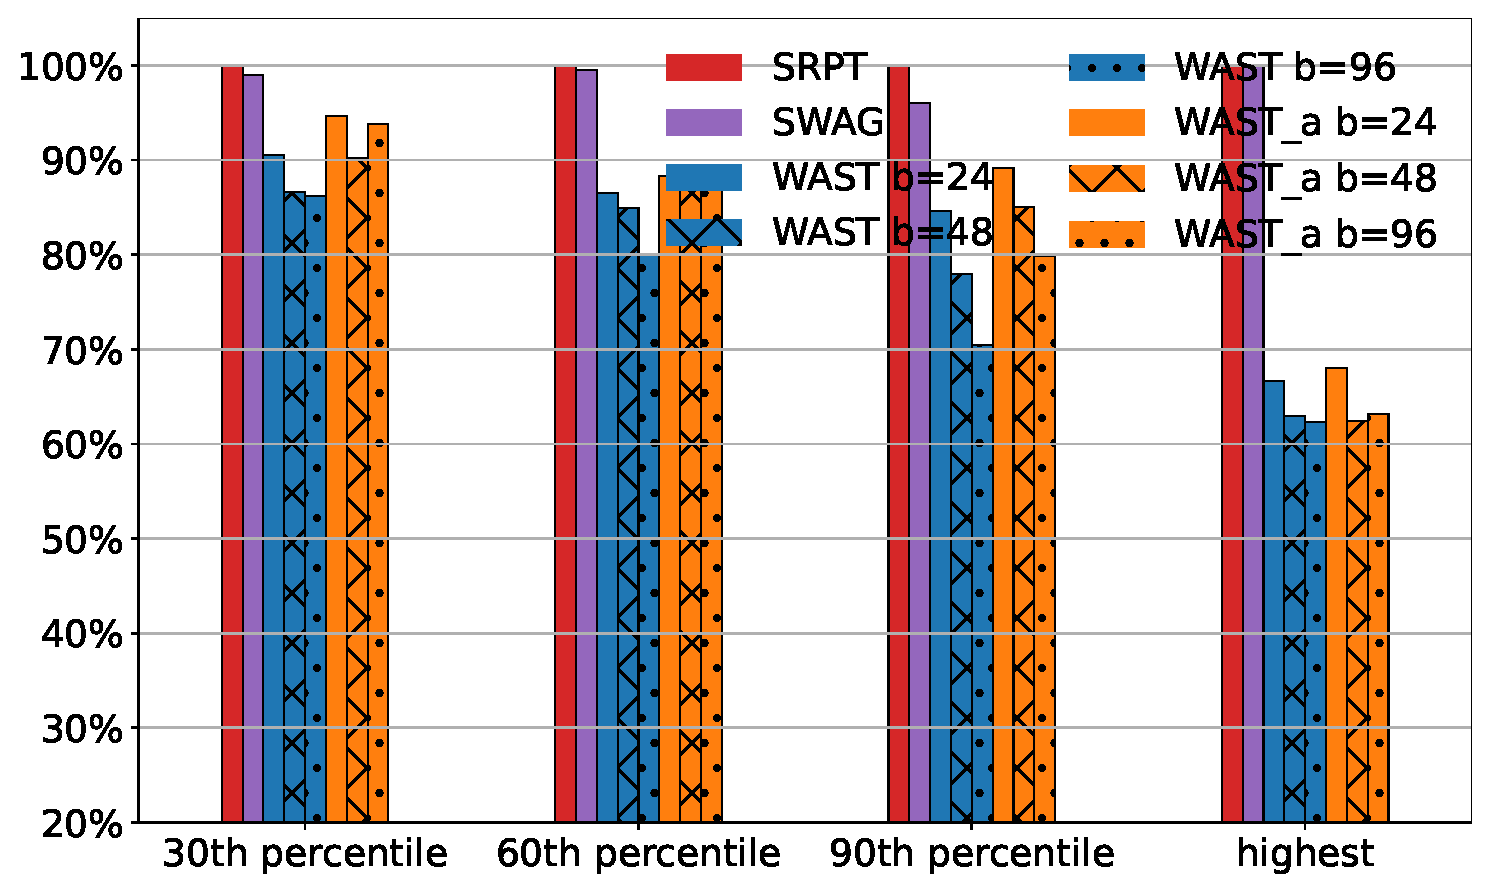
\includegraphics[width=0.24\textwidth]{Image2/CDFpercentile_Ali2018_4_70.eps}}%
\hfil
\subfloat[utilization = 80\%]
%
{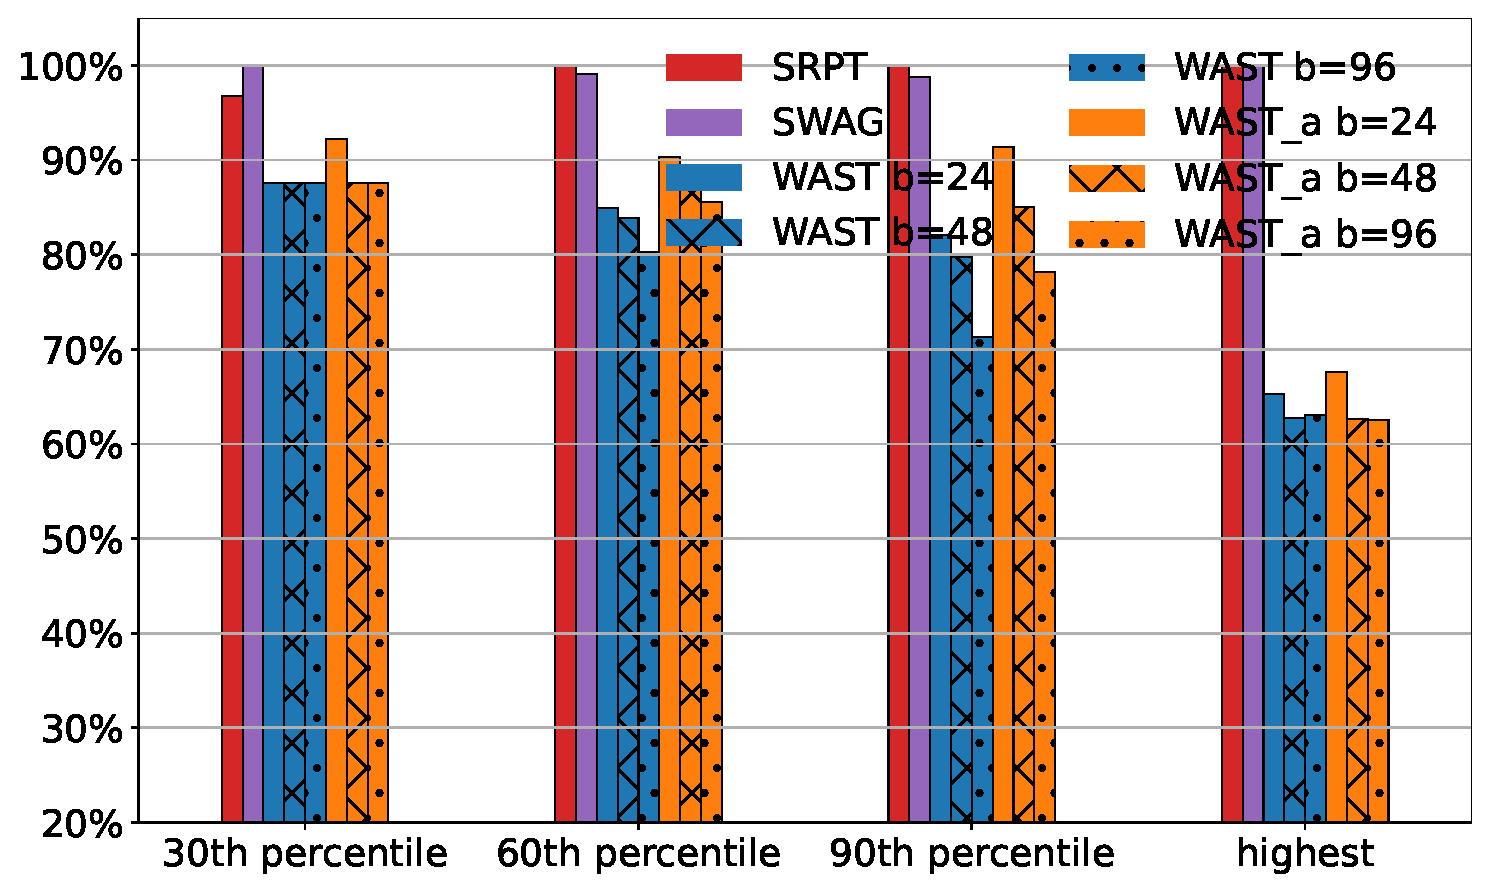
\includegraphics[width=0.24\textwidth]{Image2/CDFpercentile_Ali2018_4_80.eps}
%\label{Fg:eg2}
}
\caption{Job Response Time at Different Percentiles, Zipf Distribution $\alpha=1$, Alibaba 2018}
\label{fig:JRT_CDF2}
\end{figure*}

Tables \ref{tab:computation_time1} and \ref{tab:computation_time2} show the average computation time per recomputation of the SWAG, WAST and WAST\_a algorithms under various bandwidth settings, slot numbers per site, Zipf parameters $\alpha$ and system utilization. Due to space limitations, we present the results for the Alibaba 2018 trace under $60\%$ and $80\%$ utilization only. Both tables demonstrate that WAST\_a effectively reduces the computation time compared with WAST, which can be up to $87.3\%$. Furthermore, it can be seen that the average computation time of WAST is about an order of magnitude higher than that of SWAG, while the average computation time of WAST\_a is of the same order of magnitude as SWAG, demonstrating the effectiveness of WAST\_a in practice. %\textcolor{red}{We evaluated the computation time of both algorithms under different numbers of computing slots per server. The outcome shows that }% Under the $80\%$ utilization, the simulated duration from the first job's arrival to the last job's completion amounts to around 1.34 million seconds for the Alibaba 2017 trace and 0.4 million seconds for the Alibaba 2018 trace. In addition, the ratio of the average computation time to the average task duration is $1.1\%/0.4\%$ for two datasets in $80\%$ utilization and $0.4\%/0.2\%$ in $60\%$. This implies that during a single computation of WAST, the probability that a task execution finishes is very low. Taking the above factors together with the observation that the arrival of a new job generally has a trivial impact on the scheduling and transmission decision, we contend that the computational overhead of the WAST remains within an acceptable range, and preserving the existing job execution order and task transmission during the recomputation is a viable approach to mitigate the impact of this time cost.
%Therefore, we argue that the computation time of the algorithm has a negligible impact on the overall execution of the distributed system.

%The improvement becomes more pronounced when the workload distribution of jobs across sites is more skewed and when higher bandwidth is available, as the network resource can be more effectively utilized to mitigate job workload imbalances under these conditions. Moreover, the algorithm exhibits better performance on the Alibaba 2017 trace. This is attributable to the higher ratio of average task duration to average data partition size in 2017, which allows a greater number of tasks to be transmitted within the average task processing time, thereby providing additional opportunities to reduce job response time through task migration. Furthermore, the higher average task count per job in 2017 implies that, under highly uneven task distributions, more workload accumulates at individual sites, leading to increased response times if task migration is not applied. This, in turn, allows the algorithm to offload more tasks from peak-load sites, further enhancing response-time performance.

\begin{table}[t]
  \caption{Average computation time (second), Alibaba 2018 trace, 60\% utilization}
  \label{tab:computation_time1}
  \centering
  \scalebox{0.8}{%
    \begin{tabular}{ccccccccc}
      \toprule
      \multicolumn{3}{c}{} & \multicolumn{2}{c}{b = 24Mbps} & \multicolumn{2}{c}{b = 48Mbps} & \multicolumn{2}{c}{b = 96Mbps}\\ 
      slot & $\alpha$ & SWAG & WAST & WAST\_a  & WAST & WAST\_a & WAST & WAST\_a\\
      \midrule
      \multirow{4}{*}{32} 
      & 0.0 &  $0.0157$ & $0.1209$ & $0.0201$ & $0.1127$ &  $0.0199$ & $0.1005$& $0.0198$ \\
      & 0.5 &  $0.0184$ & $0.1323$ & $0.0323$ & $0.1167$ &  $0.0297$ & $0.1023$& $0.0274$\\
      & 1.0 &  $0.0253$ & $0.1805$ & $0.0453$ & $0.1327$ &  $0.0468$ & $0.1301$& $0.0424$ \\
      & 2.0 &  $0.0475$ & $0.3014$& $0.0756$ & $0.2283$ &  $0.0872$ & $0.1936$& $0.0877$\\
      \midrule
      \multirow{4}{*}{64} 
      & 0.0 &  $0.0306$ & $0.2293$& $0.0378$ & $0.2310$ &  $0.0399$ & $0.2283$ & $0.0376$\\
      & 0.5 & $0.0365$ & $0.2797$& $0.0585$ & $0.2467$ & $0.0653$ & $0.2330$& $0.0563$\\
      & 1.0 & $0.0502$ & $0.3646$ & $0.0883$ & $0.3281$ & $0.0781$ & $0.2867$& $0.0845$\\
      & 2.0 & $0.0885$ & $0.6217$& $0.1666$ & $0.5365$ & $0.1299$ & $0.4369$& $0.1482$\\
      \midrule
      \multirow{4}{*}{128} 
      & 0.0 &  $0.0772$ & $0.6290$& $0.0899$ & $0.6169$ &  $0.0928$ & $0.6057$& $0.0922$\\
      & 0.5 & $0.0876$ & $0.7265$& $0.1127$ & $0.7205$ & $0.1228$ & $0.6601$& $0.1341$\\
      & 1.0 & $0.1302$ & $0.9427$& $0.1459$ & $0.9012$ & $0.1565$ & $0.8432$& $0.1781$\\
      & 2.0 & $0.2068$ & $1.5751$& $0.2247$ & $1.4975$ & $0.2317$ & $1.3203$& $0.2493$\\
      \bottomrule
    \end{tabular}
    }
\end{table}

\begin{table}[t]
  \caption{Average computation time (second), Alibaba 2018 trace, 80\% utilization}
  \label{tab:computation_time2}
  \centering
  \scalebox{0.8}{%
    \begin{tabular}{ccccccccc}
      \toprule
      \multicolumn{3}{c}{} & \multicolumn{2}{c}{b = 24Mbps} & \multicolumn{2}{c}{b = 48Mbps} & \multicolumn{2}{c}{b = 96Mbps}\\ 
      slot & $\alpha$ & SWAG & WAST & WAST\_a  & WAST & WAST\_a & WAST & WAST\_a\\
      \midrule
      \multirow{4}{*}{32} 
      & 0.0 &  $0.0326$ & $0.2950$ & $0.0411$ & $0.2782$ &  $0.0398$ & $0.2543$ & $0.0393$\\
      & 0.5 &  $0.0402$ & $0.3212$ & $0.0785$ & $0.2879$ &  $0.0616$ & $0.2549$ & $0.0547$\\
      & 1.0 &  $0.0521$ & $0.4283$ & $0.1078$ & $0.3196$ &  $0.1100$ & $0.2513$ & $0.0905$\\
      & 2.0 &  $0.0964$ & $0.4826$& $0.1503$ & $0.5172$ &  $0.1785$ & $0.4501$ & $0.1746$\\
      \midrule
      \multirow{4}{*}{64} 
      & 0.0 &  $0.0667$ & $0.5337$& $0.0863$ & $0.5363$ &  $0.0891$ & $0.5340$ & $0.0818$\\
      & 0.5 & $0.0842$ & $0.6638$& $0.1378$ & $0.5871$ & $0.1483$ & $0.5706$ & $0.1266$\\
      & 1.0 & $0.1078$ & $0.8532$ & $0.2476$ & $0.7262$ & $0.1848$ & $0.6623$ & $0.2028$\\
      & 2.0 & $0.1816$ & $1.2361$& $0.3728$ & $1.1003$ & $0.2484$ & $0.9437$ & $0.2913$\\
      \midrule
      \multirow{4}{*}{128} 
      & 0.0 &  $0.1665$ & $1.3935$& $0.1963$ & $1.4098$ &  $0.2024$ & $1.4332$ & $0.2087$\\
      & 0.5 & $0.1947$ & $1.7591$& $0.2664$ & $1.6433$ & $0.2899$ & $1.6000$ & $0.3193$\\
      & 1.0 & $0.2715$ & $2.1885$& $0.3210$ & $2.0776$ & $0.3473$ & $1.8640$ & $0.3722$\\
      & 2.0 & $0.4260$ & $3.9332$& $0.4998$ & $3.6373$ & $0.5136$ & $3.0193$ & $0.5459$\\
      \bottomrule
    \end{tabular}
    }
\end{table}

\subsection{Evaluation on Robustness and Scalability}


\section{Discussion}
\textbf{Heterogeneous tasks.} In real-world workloads, a job may consist of tasks with heterogeneous processing times and data sizes. Our proposed model and algorithms are capable of handling heterogeneous tasks by replacing the parameters $l_k$ and $d_k$ with task-specific values. Although this complicates the modeling of computation and transmission process, it does not compromise the effectiveness of our proposed algorithms.

\textbf{Limited network resources.} Inter-datacenter bandwidth is often limited and costly compared to intra-datacenter links. Therefore, the scheduler must avoid excessive network resource consumption. We suggest that the algorithm should exclusively utilize the spare network bandwidth, which is identified based on current system conditions. The specific method for quantifying this spare bandwidth via network monitoring is beyond the scope of this paper.

\textbf{Replicated data inputs.} Cloud-based environments often replicate data chunks across multiple geo-distributed servers in order to reduce service response latency and data transfer overhead \cite{guan2022task, zhao2025data}. Our method can be integrated with algorithms that determine task assignments under replicated data inputs. Specifically, we first execute the task assignment algorithm to determine an initial execution site for each task, and then employ our proposed algorithm(s) to derive the job execution order and task transmissions. Notably, if a destination site is found to already host a replica of the required data partition, the corresponding transmission is not needed, and the task can be processed locally at the destination.

\section{Summary}
\label{sec:conclusion2}
In this chapter, we have proposed a WAST algorithm and a fast approximation to improve job scheduling efficiency in geo-distributed systems with the usage of network resources. WAST constructs a near-optimal job execution order with task transmissions progressively. In each round, WAST searches for the job with the minimum completion time among all unsettled jobs given the scheduled workloads and task transmissions of previous rounds. The sub-problem of minimizing a single job's completion time is converted into solving multiple minimum-cost flow problems, which can be computed efficiently. 
%Once the job is found, its computation load and transmissions are updated to the system, and the next round starts with the updated system computing and network resource usage conditions. The process repeats until all jobs are scheduled. 
We also present a fast approximation to WAST, which optimizes each job's completion time by transferring its tasks of the latest completion time to other sites recursively. We have evaluated WAST and its approximation using real job traces from Alibaba. The experimental results show that WAST can effectively reduce the average job response time, especially when the task distributions of jobs are highly skewed.